\documentclass[twoside]{book}

% Packages required by doxygen
\usepackage{fixltx2e}
\usepackage{calc}
\usepackage{doxygen}
\usepackage[export]{adjustbox} % also loads graphicx
\usepackage{graphicx}
\usepackage[utf8]{inputenc}
\usepackage{makeidx}
\usepackage{multicol}
\usepackage{multirow}
\PassOptionsToPackage{warn}{textcomp}
\usepackage{textcomp}
\usepackage[nointegrals]{wasysym}
\usepackage[table]{xcolor}

% Font selection
\usepackage[T1]{fontenc}
\usepackage[scaled=.90]{helvet}
\usepackage{courier}
\usepackage{amssymb}
\usepackage{sectsty}
\renewcommand{\familydefault}{\sfdefault}
\allsectionsfont{%
  \fontseries{bc}\selectfont%
  \color{darkgray}%
}
\renewcommand{\DoxyLabelFont}{%
  \fontseries{bc}\selectfont%
  \color{darkgray}%
}
\newcommand{\+}{\discretionary{\mbox{\scriptsize$\hookleftarrow$}}{}{}}

% Page & text layout
\usepackage{geometry}
\geometry{%
  a4paper,%
  top=2.5cm,%
  bottom=2.5cm,%
  left=2.5cm,%
  right=2.5cm%
}
\tolerance=750
\hfuzz=15pt
\hbadness=750
\setlength{\emergencystretch}{15pt}
\setlength{\parindent}{0cm}
\setlength{\parskip}{3ex plus 2ex minus 2ex}
\makeatletter
\renewcommand{\paragraph}{%
  \@startsection{paragraph}{4}{0ex}{-1.0ex}{1.0ex}{%
    \normalfont\normalsize\bfseries\SS@parafont%
  }%
}
\renewcommand{\subparagraph}{%
  \@startsection{subparagraph}{5}{0ex}{-1.0ex}{1.0ex}{%
    \normalfont\normalsize\bfseries\SS@subparafont%
  }%
}
\makeatother

% Headers & footers
\usepackage{fancyhdr}
\pagestyle{fancyplain}
\fancyhead[LE]{\fancyplain{}{\bfseries\thepage}}
\fancyhead[CE]{\fancyplain{}{}}
\fancyhead[RE]{\fancyplain{}{\bfseries\leftmark}}
\fancyhead[LO]{\fancyplain{}{\bfseries\rightmark}}
\fancyhead[CO]{\fancyplain{}{}}
\fancyhead[RO]{\fancyplain{}{\bfseries\thepage}}
\fancyfoot[LE]{\fancyplain{}{}}
\fancyfoot[CE]{\fancyplain{}{}}
\fancyfoot[RE]{\fancyplain{}{\bfseries\scriptsize Generated by Doxygen }}
\fancyfoot[LO]{\fancyplain{}{\bfseries\scriptsize Generated by Doxygen }}
\fancyfoot[CO]{\fancyplain{}{}}
\fancyfoot[RO]{\fancyplain{}{}}
\renewcommand{\footrulewidth}{0.4pt}
\renewcommand{\chaptermark}[1]{%
  \markboth{#1}{}%
}
\renewcommand{\sectionmark}[1]{%
  \markright{\thesection\ #1}%
}

% Indices & bibliography
\usepackage{natbib}
\usepackage[titles]{tocloft}
\setcounter{tocdepth}{3}
\setcounter{secnumdepth}{5}
\makeindex

% Hyperlinks (required, but should be loaded last)
\usepackage{ifpdf}
\ifpdf
  \usepackage[pdftex,pagebackref=true]{hyperref}
\else
  \usepackage[ps2pdf,pagebackref=true]{hyperref}
\fi
\hypersetup{%
  colorlinks=true,%
  linkcolor=blue,%
  citecolor=blue,%
  unicode%
}

% Custom commands
\newcommand{\clearemptydoublepage}{%
  \newpage{\pagestyle{empty}\cleardoublepage}%
}

\usepackage{caption}
\captionsetup{labelsep=space,justification=centering,font={bf},singlelinecheck=off,skip=4pt,position=top}

%===== C O N T E N T S =====

\begin{document}

% Titlepage & ToC
\hypersetup{pageanchor=false,
             bookmarksnumbered=true,
             pdfencoding=unicode
            }
\pagenumbering{roman}
\begin{titlepage}
\vspace*{7cm}
\begin{center}%
{\Large Team\+Speak3-\/\+C-\/\+Query-\/\+A\+PI \\[1ex]\large 0.\+1a }\\
\vspace*{1cm}
{\large Generated by Doxygen 1.8.11}\\
\end{center}
\end{titlepage}
\clearemptydoublepage
\tableofcontents
\clearemptydoublepage
\pagenumbering{arabic}
\hypersetup{pageanchor=true}

%--- Begin generated contents ---
\chapter{Namespace Index}
\section{Namespace List}
Here is a list of all documented namespaces with brief descriptions\+:\begin{DoxyCompactList}
\item\contentsline{section}{\hyperlink{namespace_ts3_api}{Ts3\+Api} }{\pageref{namespace_ts3_api}}{}
\end{DoxyCompactList}

\chapter{Hierarchical Index}
\section{Hierarchia klas}
Ta lista dziedziczenia posortowana jest z grubsza, choć nie całkowicie, alfabetycznie\+:\begin{DoxyCompactList}
\item \contentsline{section}{Ts3\+Api\+:\+:Client\+:\+:changeable\+Param}{\pageref{struct_ts3_api_1_1_client_1_1changeable_param}}{}
\item \contentsline{section}{Ts3\+Api\+:\+:Channel}{\pageref{class_ts3_api_1_1_channel}}{}
\item \contentsline{section}{Ts3\+Api\+:\+:Client}{\pageref{class_ts3_api_1_1_client}}{}
\item \contentsline{section}{Ts3\+Api\+:\+:Client\+:\+:connection\+Info}{\pageref{struct_ts3_api_1_1_client_1_1connection_info}}{}
\item \contentsline{section}{Ts3\+Api\+:\+:error}{\pageref{struct_ts3_api_1_1error}}{}
\item \contentsline{section}{Ts3\+Api\+:\+:Group}{\pageref{class_ts3_api_1_1_group}}{}
\item \contentsline{section}{Ts3\+Api\+:\+:Client\+:\+:I\+Ds}{\pageref{struct_ts3_api_1_1_client_1_1_i_ds}}{}
\item \contentsline{section}{Ts3\+Api\+:\+:Client\+:\+:nickname}{\pageref{struct_ts3_api_1_1_client_1_1nickname}}{}
\item \contentsline{section}{Ts3\+Api\+:\+:Permission}{\pageref{class_ts3_api_1_1_permission}}{}
\item \contentsline{section}{Ts3\+Api\+:\+:Client\+:\+:properties}{\pageref{struct_ts3_api_1_1_client_1_1properties}}{}
\begin{DoxyCompactList}
\item \contentsline{section}{Ts3\+Api\+:\+:Client\+:\+:client\+Info\+Properties}{\pageref{struct_ts3_api_1_1_client_1_1client_info_properties}}{}
\end{DoxyCompactList}
\item \contentsline{section}{Ts3\+Api\+:\+:Client\+:\+:property}{\pageref{struct_ts3_api_1_1_client_1_1property}}{}
\item \contentsline{section}{Ts3\+Api\+:\+:Server}{\pageref{class_ts3_api_1_1_server}}{}
\item \contentsline{section}{Ts3\+Api\+:\+:socket\+Data}{\pageref{struct_ts3_api_1_1socket_data}}{}
\item \contentsline{section}{Ts3\+Api\+:\+:timestamp\+Time}{\pageref{struct_ts3_api_1_1timestamp_time}}{}
\item \contentsline{section}{Ts3\+Api\+:\+:Client\+:\+:transfer\+Info}{\pageref{struct_ts3_api_1_1_client_1_1transfer_info}}{}
\item \contentsline{section}{Ts3\+Api\+:\+:ts3\+Response}{\pageref{struct_ts3_api_1_1ts3_response}}{}
\end{DoxyCompactList}

\chapter{Class Index}
\section{Class List}
Here are the classes, structs, unions and interfaces with brief descriptions\+:\begin{DoxyCompactList}
\item\contentsline{section}{\hyperlink{struct_ts3_api_1_1_client_1_1changeable_param}{Ts3\+Api\+::\+Client\+::changeable\+Param} \\*Struktura pozwala na sprawdzenie oraz zmianę wybranej właściwości użytkownika }{\pageref{struct_ts3_api_1_1_client_1_1changeable_param}}{}
\item\contentsline{section}{\hyperlink{class_ts3_api_1_1_channel}{Ts3\+Api\+::\+Channel} \\*Class for channel }{\pageref{class_ts3_api_1_1_channel}}{}
\item\contentsline{section}{\hyperlink{struct_ts3_api_1_1_channel_1_1channel_changeable_param}{Ts3\+Api\+::\+Channel\+::channel\+Changeable\+Param} \\*Providing possibility to change selected param }{\pageref{struct_ts3_api_1_1_channel_1_1channel_changeable_param}}{}
\item\contentsline{section}{\hyperlink{struct_ts3_api_1_1_channel_1_1channel_codec}{Ts3\+Api\+::\+Channel\+::channel\+Codec} \\*Contain channel codec settings }{\pageref{struct_ts3_api_1_1_channel_1_1channel_codec}}{}
\item\contentsline{section}{\hyperlink{struct_ts3_api_1_1_channel_1_1channel_flags}{Ts3\+Api\+::\+Channel\+::channel\+Flags} \\*Contain channel flags }{\pageref{struct_ts3_api_1_1_channel_1_1channel_flags}}{}
\item\contentsline{section}{\hyperlink{struct_ts3_api_1_1_channel_1_1channel_name}{Ts3\+Api\+::\+Channel\+::channel\+Name} \\*Contain channel names }{\pageref{struct_ts3_api_1_1_channel_1_1channel_name}}{}
\item\contentsline{section}{\hyperlink{class_ts3_api_1_1_client}{Ts3\+Api\+::\+Client} \\*Pozwala na manupulacje wybranym użytkownikiem }{\pageref{class_ts3_api_1_1_client}}{}
\item\contentsline{section}{\hyperlink{struct_ts3_api_1_1_client_1_1client_info_properties}{Ts3\+Api\+::\+Client\+::client\+Info\+Properties} \\*Struktura zawierająca informacje z polecenia query\+: \char`\"{}clientinfo\char`\"{} }{\pageref{struct_ts3_api_1_1_client_1_1client_info_properties}}{}
\item\contentsline{section}{\hyperlink{struct_ts3_api_1_1_client_1_1connection_info}{Ts3\+Api\+::\+Client\+::connection\+Info} \\*Zawiera informacje o połączeniu danego użykownika }{\pageref{struct_ts3_api_1_1_client_1_1connection_info}}{}
\item\contentsline{section}{\hyperlink{struct_ts3_api_1_1error}{Ts3\+Api\+::error} }{\pageref{struct_ts3_api_1_1error}}{}
\item\contentsline{section}{\hyperlink{class_ts3_api_1_1_group}{Ts3\+Api\+::\+Group} }{\pageref{class_ts3_api_1_1_group}}{}
\item\contentsline{section}{\hyperlink{struct_ts3_api_1_1_client_1_1_i_ds}{Ts3\+Api\+::\+Client\+::\+I\+Ds} \\*Zbiór indentyfikatorów użytkownika }{\pageref{struct_ts3_api_1_1_client_1_1_i_ds}}{}
\item\contentsline{section}{\hyperlink{struct_ts3_api_1_1_client_1_1nickname}{Ts3\+Api\+::\+Client\+::nickname} }{\pageref{struct_ts3_api_1_1_client_1_1nickname}}{}
\item\contentsline{section}{\hyperlink{class_ts3_api_1_1_permission}{Ts3\+Api\+::\+Permission} }{\pageref{class_ts3_api_1_1_permission}}{}
\item\contentsline{section}{\hyperlink{struct_ts3_api_1_1property}{Ts3\+Api\+::property} }{\pageref{struct_ts3_api_1_1property}}{}
\item\contentsline{section}{\hyperlink{class_ts3_api_1_1_server}{Ts3\+Api\+::\+Server} \\*\hyperlink{class_ts3_api_1_1_server}{Server} Class }{\pageref{class_ts3_api_1_1_server}}{}
\item\contentsline{section}{\hyperlink{struct_ts3_api_1_1socket_data}{Ts3\+Api\+::socket\+Data} }{\pageref{struct_ts3_api_1_1socket_data}}{}
\item\contentsline{section}{\hyperlink{struct_ts3_api_1_1timestamp_time}{Ts3\+Api\+::timestamp\+Time} \\*Pozwala odczytać datę zapisaną w formacie timestamp }{\pageref{struct_ts3_api_1_1timestamp_time}}{}
\item\contentsline{section}{\hyperlink{struct_ts3_api_1_1_client_1_1transfer_info}{Ts3\+Api\+::\+Client\+::transfer\+Info} \\*Zawiera informacje o transferze dengo użytkownika }{\pageref{struct_ts3_api_1_1_client_1_1transfer_info}}{}
\item\contentsline{section}{\hyperlink{struct_ts3_api_1_1ts3_object_properties}{Ts3\+Api\+::ts3\+Object\+Properties} }{\pageref{struct_ts3_api_1_1ts3_object_properties}}{}
\item\contentsline{section}{\hyperlink{struct_ts3_api_1_1ts3_response}{Ts3\+Api\+::ts3\+Response} }{\pageref{struct_ts3_api_1_1ts3_response}}{}
\end{DoxyCompactList}

\chapter{Namespace Documentation}
\hypertarget{namespace_ts3_api}{}\section{Ts3\+Api Namespace Reference}
\label{namespace_ts3_api}\index{Ts3\+Api@{Ts3\+Api}}
\subsection*{Classes}
\begin{DoxyCompactItemize}
\item 
class \hyperlink{class_ts3_api_1_1_channel}{Channel}
\begin{DoxyCompactList}\small\item\em Class for channel. \end{DoxyCompactList}\item 
class \hyperlink{class_ts3_api_1_1_client}{Client}
\begin{DoxyCompactList}\small\item\em Pozwala na manupulacje wybranym użytkownikiem. \end{DoxyCompactList}\item 
struct \hyperlink{struct_ts3_api_1_1error}{error}
\item 
class \hyperlink{class_ts3_api_1_1_group}{Group}
\item 
class \hyperlink{class_ts3_api_1_1_permission}{Permission}
\item 
struct \hyperlink{struct_ts3_api_1_1property}{property}
\item 
class \hyperlink{class_ts3_api_1_1_server}{Server}
\begin{DoxyCompactList}\small\item\em \hyperlink{class_ts3_api_1_1_server}{Server} Class. \end{DoxyCompactList}\item 
struct \hyperlink{struct_ts3_api_1_1socket_data}{socket\+Data}
\item 
struct \hyperlink{struct_ts3_api_1_1timestamp_time}{timestamp\+Time}
\begin{DoxyCompactList}\small\item\em Pozwala odczytać datę zapisaną w formacie timestamp. \end{DoxyCompactList}\item 
struct \hyperlink{struct_ts3_api_1_1ts3_object_properties}{ts3\+Object\+Properties}
\item 
struct \hyperlink{struct_ts3_api_1_1ts3_response}{ts3\+Response}
\end{DoxyCompactItemize}
\subsection*{Functions}
\begin{DoxyCompactItemize}
\item 
string {\bfseries message\+Encode} (string message)\hypertarget{namespace_ts3_api_aced196e110a77c44616fbe90d94edc7e}{}\label{namespace_ts3_api_aced196e110a77c44616fbe90d94edc7e}

\item 
string {\bfseries message\+Decode} (string message)\hypertarget{namespace_ts3_api_ad21f5397ccc853661d734146598da547}{}\label{namespace_ts3_api_ad21f5397ccc853661d734146598da547}

\item 
void {\bfseries split} (map$<$ string, string $>$ \&returned\+Map, string input)\hypertarget{namespace_ts3_api_a07703eef88c4288a04dd84ff342b073b}{}\label{namespace_ts3_api_a07703eef88c4288a04dd84ff342b073b}

\item 
void {\bfseries split} (map$<$ string, map$<$ string, string $>$$>$ \&returned\+Map, string input, string map\+Index=\char`\"{}intiger\char`\"{})\hypertarget{namespace_ts3_api_a99c4f893b8ac36a7d5bb713b7bceda2f}{}\label{namespace_ts3_api_a99c4f893b8ac36a7d5bb713b7bceda2f}

\end{DoxyCompactItemize}


\subsection{Detailed Description}
Zawiera wszystkie elementy A\+PI 
\chapter{Class Documentation}
\hypertarget{struct_ts3_api_1_1_client_1_1changeable_param}{}\section{Dokumentacja struktury Ts3\+Api\+:\+:Client\+:\+:changeable\+Param}
\label{struct_ts3_api_1_1_client_1_1changeable_param}\index{Ts3\+Api\+::\+Client\+::changeable\+Param@{Ts3\+Api\+::\+Client\+::changeable\+Param}}
\subsection*{Metody publiczne}
\begin{DoxyCompactItemize}
\item 
{\bfseries changeable\+Param} (\hyperlink{class_ts3_api_1_1_client}{Client} \&client, string value, string param\+Name)\hypertarget{struct_ts3_api_1_1_client_1_1changeable_param_a1e378b376136300d1420542efc1e7e5d}{}\label{struct_ts3_api_1_1_client_1_1changeable_param_a1e378b376136300d1420542efc1e7e5d}

\item 
\hyperlink{struct_ts3_api_1_1ts3_response}{ts3\+Response} {\bfseries change} (string value)\hypertarget{struct_ts3_api_1_1_client_1_1changeable_param_ac3f3dd298ba1d2c0d5db342217c891af}{}\label{struct_ts3_api_1_1_client_1_1changeable_param_ac3f3dd298ba1d2c0d5db342217c891af}

\end{DoxyCompactItemize}
\subsection*{Atrybuty publiczne}
\begin{DoxyCompactItemize}
\item 
string {\bfseries value}\hypertarget{struct_ts3_api_1_1_client_1_1changeable_param_a4e3b8780f19688a682dc08e3e15912a3}{}\label{struct_ts3_api_1_1_client_1_1changeable_param_a4e3b8780f19688a682dc08e3e15912a3}

\end{DoxyCompactItemize}


Dokumentacja dla tej struktury została wygenerowana z plików\+:\begin{DoxyCompactItemize}
\item 
/home/karol/projects/ts3\+A\+P\+Iv2/src/includes/Client.\+hpp\item 
/home/karol/projects/ts3\+A\+P\+Iv2/src/Client.\+cpp\end{DoxyCompactItemize}

\hypertarget{class_ts3_api_1_1_channel}{}\section{Ts3\+Api\+:\+:Channel Class Reference}
\label{class_ts3_api_1_1_channel}\index{Ts3\+Api\+::\+Channel@{Ts3\+Api\+::\+Channel}}


Class for channel.  




{\ttfamily \#include $<$Channel.\+hpp$>$}

\subsection*{Classes}
\begin{DoxyCompactItemize}
\item 
struct \hyperlink{struct_ts3_api_1_1_channel_1_1channel_changeable_param}{channel\+Changeable\+Param}
\begin{DoxyCompactList}\small\item\em Providing possibility to change selected param. \end{DoxyCompactList}\item 
struct \hyperlink{struct_ts3_api_1_1_channel_1_1channel_codec}{channel\+Codec}
\begin{DoxyCompactList}\small\item\em Contain channel codec settings. \end{DoxyCompactList}\item 
struct \hyperlink{struct_ts3_api_1_1_channel_1_1channel_flags}{channel\+Flags}
\begin{DoxyCompactList}\small\item\em Contain channel flags. \end{DoxyCompactList}\item 
struct \hyperlink{struct_ts3_api_1_1_channel_1_1channel_name}{channel\+Name}
\begin{DoxyCompactList}\small\item\em Contain channel names. \end{DoxyCompactList}\end{DoxyCompactItemize}
\subsection*{Public Member Functions}
\begin{DoxyCompactItemize}
\item 
{\bfseries Channel} (\hyperlink{class_ts3_api_1_1_server}{Server} \&server, string id, bool incomlete\+Init=false)\hypertarget{class_ts3_api_1_1_channel_a6b09dc4ce2d937ef2e9c5be0a1f6f921}{}\label{class_ts3_api_1_1_channel_a6b09dc4ce2d937ef2e9c5be0a1f6f921}

\item 
void \hyperlink{class_ts3_api_1_1_channel_a46a6b75a6034ebac72a4868ed943ad05}{update} ()\hypertarget{class_ts3_api_1_1_channel_a46a6b75a6034ebac72a4868ed943ad05}{}\label{class_ts3_api_1_1_channel_a46a6b75a6034ebac72a4868ed943ad05}

\begin{DoxyCompactList}\small\item\em Forces to updata data with next get Action. \end{DoxyCompactList}\item 
\hyperlink{struct_ts3_api_1_1_channel_1_1channel_changeable_param}{channel\+Changeable\+Param} \hyperlink{class_ts3_api_1_1_channel_a563ae891e7c032d78598fc6463c0c116}{get\+Pid} ()
\begin{DoxyCompactList}\small\item\em Gets the channel parent ID. \end{DoxyCompactList}\item 
\hyperlink{struct_ts3_api_1_1_channel_1_1channel_name}{channel\+Name} \hyperlink{class_ts3_api_1_1_channel_a3652d653afd949b86a644d0313343e76}{get\+Name} ()
\begin{DoxyCompactList}\small\item\em Gets the channel name. \end{DoxyCompactList}\item 
\hyperlink{struct_ts3_api_1_1_channel_1_1channel_changeable_param}{channel\+Changeable\+Param} \hyperlink{class_ts3_api_1_1_channel_a1f0389083a67195ccd2c74097588e44f}{get\+Topic} ()
\begin{DoxyCompactList}\small\item\em Gets the channel topic. \end{DoxyCompactList}\item 
\hyperlink{struct_ts3_api_1_1_channel_1_1channel_changeable_param}{channel\+Changeable\+Param} \hyperlink{class_ts3_api_1_1_channel_a44b6339c1b2103561ea66a6f63a213dd}{get\+Description} ()
\begin{DoxyCompactList}\small\item\em Gets the channel description. \end{DoxyCompactList}\item 
\hyperlink{struct_ts3_api_1_1_channel_1_1channel_changeable_param}{channel\+Changeable\+Param} \hyperlink{class_ts3_api_1_1_channel_a28058f3c4691d52414fa148075d2a854}{get\+Password} ()
\begin{DoxyCompactList}\small\item\em Gets the channel password. \end{DoxyCompactList}\item 
\hyperlink{struct_ts3_api_1_1_channel_1_1channel_codec}{channel\+Codec} \hyperlink{class_ts3_api_1_1_channel_a354ec6ea657cf69f54e4593c6a952973}{get\+Codec} ()
\begin{DoxyCompactList}\small\item\em Gets the channel codec settings. \end{DoxyCompactList}\item 
\hyperlink{struct_ts3_api_1_1_channel_1_1channel_changeable_param}{channel\+Changeable\+Param} \hyperlink{class_ts3_api_1_1_channel_af1c732fc3662583b5f1a27df09c31225}{get\+Max\+Clients} ()
\begin{DoxyCompactList}\small\item\em Gets the maximum channel clients. \end{DoxyCompactList}\item 
\hyperlink{struct_ts3_api_1_1_channel_1_1channel_changeable_param}{channel\+Changeable\+Param} \hyperlink{class_ts3_api_1_1_channel_a4b77cc2a599ca9c8f535fdd22a9826f9}{get\+Max\+Family\+Clients} ()
\begin{DoxyCompactList}\small\item\em Gets the channem maximum family clients. \end{DoxyCompactList}\item 
\hyperlink{struct_ts3_api_1_1_channel_1_1channel_changeable_param}{channel\+Changeable\+Param} \hyperlink{class_ts3_api_1_1_channel_a4eef83062ec9df4f2e66cb399ee9a916}{get\+Order} ()
\begin{DoxyCompactList}\small\item\em Gets the channel order ID. \end{DoxyCompactList}\item 
\hyperlink{struct_ts3_api_1_1_channel_1_1channel_flags}{channel\+Flags} \hyperlink{class_ts3_api_1_1_channel_ae2d7acea0b808965a7ce9001e1b13dcb}{get\+Flags} ()
\begin{DoxyCompactList}\small\item\em Gets the channel flagsflags. \end{DoxyCompactList}\item 
\hyperlink{struct_ts3_api_1_1property}{property} \hyperlink{class_ts3_api_1_1_channel_a971cf9d6ed8759120ed68319922fc028}{get\+Security\+Salt} ()
\begin{DoxyCompactList}\small\item\em Gets the channel secutiry salt. \end{DoxyCompactList}\item 
\hyperlink{struct_ts3_api_1_1property}{property} \hyperlink{class_ts3_api_1_1_channel_a760b3a902325a34d9e82ff49946535a9}{get\+Delete\+Delay} ()
\begin{DoxyCompactList}\small\item\em Gets the channel delete delay. \end{DoxyCompactList}\item 
\hyperlink{struct_ts3_api_1_1property}{property} \hyperlink{class_ts3_api_1_1_channel_a2e9efe39dddfa4ef8e39774269525bce}{get\+Filepath} ()
\begin{DoxyCompactList}\small\item\em Gets the channel filepath. \end{DoxyCompactList}\item 
\hyperlink{struct_ts3_api_1_1_channel_1_1channel_changeable_param}{channel\+Changeable\+Param} \hyperlink{class_ts3_api_1_1_channel_ab38a596734ecc93a019c4aa50b4324c5}{get\+Need\+Talk\+Power} ()
\begin{DoxyCompactList}\small\item\em Gets the channel need talk power. \end{DoxyCompactList}\item 
\hyperlink{struct_ts3_api_1_1property}{property} \hyperlink{class_ts3_api_1_1_channel_a0dbe0383820514a042d27ac38cbb5cce}{get\+Forced\+Silence} ()
\begin{DoxyCompactList}\small\item\em Gets the channel forced silence. \end{DoxyCompactList}\item 
\hyperlink{struct_ts3_api_1_1_channel_1_1channel_changeable_param}{channel\+Changeable\+Param} \hyperlink{class_ts3_api_1_1_channel_a23be361507d0eb269c84c736e3501c07}{get\+Icon\+Id} ()
\begin{DoxyCompactList}\small\item\em Gets the icon identifier. \end{DoxyCompactList}\item 
\hyperlink{struct_ts3_api_1_1property}{property} \hyperlink{class_ts3_api_1_1_channel_afbaae870da911877f6c39795e685fa17}{get\+Seconds\+Empty} ()
\begin{DoxyCompactList}\small\item\em Gets the channel seconds empty. \end{DoxyCompactList}\end{DoxyCompactItemize}
\subsection*{Friends}
\begin{DoxyCompactItemize}
\item 
class {\bfseries Client}\hypertarget{class_ts3_api_1_1_channel_a5db1c99e2c94b26278f3838c85cdb618}{}\label{class_ts3_api_1_1_channel_a5db1c99e2c94b26278f3838c85cdb618}

\item 
class {\bfseries Server}\hypertarget{class_ts3_api_1_1_channel_ac2055578ac48afabe5af487878450f68}{}\label{class_ts3_api_1_1_channel_ac2055578ac48afabe5af487878450f68}

\item 
class {\bfseries Permission}\hypertarget{class_ts3_api_1_1_channel_ad3834bbd6b2c4839e7f69dc4cc1d6ae6}{}\label{class_ts3_api_1_1_channel_ad3834bbd6b2c4839e7f69dc4cc1d6ae6}

\end{DoxyCompactItemize}


\subsection{Detailed Description}
Class for channel. 

\subsection{Member Function Documentation}
\index{Ts3\+Api\+::\+Channel@{Ts3\+Api\+::\+Channel}!get\+Codec@{get\+Codec}}
\index{get\+Codec@{get\+Codec}!Ts3\+Api\+::\+Channel@{Ts3\+Api\+::\+Channel}}
\subsubsection[{\texorpdfstring{get\+Codec()}{getCodec()}}]{\setlength{\rightskip}{0pt plus 5cm}{\bf Channel\+::channel\+Codec} Channel\+::get\+Codec (
\begin{DoxyParamCaption}
{}
\end{DoxyParamCaption}
)}\hypertarget{class_ts3_api_1_1_channel_a354ec6ea657cf69f54e4593c6a952973}{}\label{class_ts3_api_1_1_channel_a354ec6ea657cf69f54e4593c6a952973}


Gets the channel codec settings. 

\begin{DoxyReturn}{Returns}
\hyperlink{class_ts3_api_1_1_channel}{Channel} codec settings with possibility to change them 
\end{DoxyReturn}
\index{Ts3\+Api\+::\+Channel@{Ts3\+Api\+::\+Channel}!get\+Delete\+Delay@{get\+Delete\+Delay}}
\index{get\+Delete\+Delay@{get\+Delete\+Delay}!Ts3\+Api\+::\+Channel@{Ts3\+Api\+::\+Channel}}
\subsubsection[{\texorpdfstring{get\+Delete\+Delay()}{getDeleteDelay()}}]{\setlength{\rightskip}{0pt plus 5cm}{\bf property} Channel\+::get\+Delete\+Delay (
\begin{DoxyParamCaption}
{}
\end{DoxyParamCaption}
)}\hypertarget{class_ts3_api_1_1_channel_a760b3a902325a34d9e82ff49946535a9}{}\label{class_ts3_api_1_1_channel_a760b3a902325a34d9e82ff49946535a9}


Gets the channel delete delay. 

\begin{DoxyReturn}{Returns}
\hyperlink{class_ts3_api_1_1_channel}{Channel} delete delay 
\end{DoxyReturn}
\index{Ts3\+Api\+::\+Channel@{Ts3\+Api\+::\+Channel}!get\+Description@{get\+Description}}
\index{get\+Description@{get\+Description}!Ts3\+Api\+::\+Channel@{Ts3\+Api\+::\+Channel}}
\subsubsection[{\texorpdfstring{get\+Description()}{getDescription()}}]{\setlength{\rightskip}{0pt plus 5cm}{\bf Channel\+::channel\+Changeable\+Param} Channel\+::get\+Description (
\begin{DoxyParamCaption}
{}
\end{DoxyParamCaption}
)}\hypertarget{class_ts3_api_1_1_channel_a44b6339c1b2103561ea66a6f63a213dd}{}\label{class_ts3_api_1_1_channel_a44b6339c1b2103561ea66a6f63a213dd}


Gets the channel description. 

\begin{DoxyReturn}{Returns}
\hyperlink{class_ts3_api_1_1_channel}{Channel} description with possibility to change it 
\end{DoxyReturn}
\index{Ts3\+Api\+::\+Channel@{Ts3\+Api\+::\+Channel}!get\+Filepath@{get\+Filepath}}
\index{get\+Filepath@{get\+Filepath}!Ts3\+Api\+::\+Channel@{Ts3\+Api\+::\+Channel}}
\subsubsection[{\texorpdfstring{get\+Filepath()}{getFilepath()}}]{\setlength{\rightskip}{0pt plus 5cm}{\bf property} Channel\+::get\+Filepath (
\begin{DoxyParamCaption}
{}
\end{DoxyParamCaption}
)}\hypertarget{class_ts3_api_1_1_channel_a2e9efe39dddfa4ef8e39774269525bce}{}\label{class_ts3_api_1_1_channel_a2e9efe39dddfa4ef8e39774269525bce}


Gets the channel filepath. 

\begin{DoxyReturn}{Returns}
\hyperlink{class_ts3_api_1_1_channel}{Channel} filepath. 
\end{DoxyReturn}
\index{Ts3\+Api\+::\+Channel@{Ts3\+Api\+::\+Channel}!get\+Flags@{get\+Flags}}
\index{get\+Flags@{get\+Flags}!Ts3\+Api\+::\+Channel@{Ts3\+Api\+::\+Channel}}
\subsubsection[{\texorpdfstring{get\+Flags()}{getFlags()}}]{\setlength{\rightskip}{0pt plus 5cm}{\bf Channel\+::channel\+Flags} Channel\+::get\+Flags (
\begin{DoxyParamCaption}
{}
\end{DoxyParamCaption}
)}\hypertarget{class_ts3_api_1_1_channel_ae2d7acea0b808965a7ce9001e1b13dcb}{}\label{class_ts3_api_1_1_channel_ae2d7acea0b808965a7ce9001e1b13dcb}


Gets the channel flagsflags. 

\begin{DoxyReturn}{Returns}
\hyperlink{class_ts3_api_1_1_channel}{Channel} flags with possibility to change it 
\end{DoxyReturn}
\index{Ts3\+Api\+::\+Channel@{Ts3\+Api\+::\+Channel}!get\+Forced\+Silence@{get\+Forced\+Silence}}
\index{get\+Forced\+Silence@{get\+Forced\+Silence}!Ts3\+Api\+::\+Channel@{Ts3\+Api\+::\+Channel}}
\subsubsection[{\texorpdfstring{get\+Forced\+Silence()}{getForcedSilence()}}]{\setlength{\rightskip}{0pt plus 5cm}{\bf property} Channel\+::get\+Forced\+Silence (
\begin{DoxyParamCaption}
{}
\end{DoxyParamCaption}
)}\hypertarget{class_ts3_api_1_1_channel_a0dbe0383820514a042d27ac38cbb5cce}{}\label{class_ts3_api_1_1_channel_a0dbe0383820514a042d27ac38cbb5cce}


Gets the channel forced silence. 

\begin{DoxyReturn}{Returns}
\hyperlink{class_ts3_api_1_1_channel}{Channel} forced silence 
\end{DoxyReturn}
\index{Ts3\+Api\+::\+Channel@{Ts3\+Api\+::\+Channel}!get\+Icon\+Id@{get\+Icon\+Id}}
\index{get\+Icon\+Id@{get\+Icon\+Id}!Ts3\+Api\+::\+Channel@{Ts3\+Api\+::\+Channel}}
\subsubsection[{\texorpdfstring{get\+Icon\+Id()}{getIconId()}}]{\setlength{\rightskip}{0pt plus 5cm}{\bf Channel\+::channel\+Changeable\+Param} Channel\+::get\+Icon\+Id (
\begin{DoxyParamCaption}
{}
\end{DoxyParamCaption}
)}\hypertarget{class_ts3_api_1_1_channel_a23be361507d0eb269c84c736e3501c07}{}\label{class_ts3_api_1_1_channel_a23be361507d0eb269c84c736e3501c07}


Gets the icon identifier. 

\begin{DoxyReturn}{Returns}
Icon identifier 
\end{DoxyReturn}
\index{Ts3\+Api\+::\+Channel@{Ts3\+Api\+::\+Channel}!get\+Max\+Clients@{get\+Max\+Clients}}
\index{get\+Max\+Clients@{get\+Max\+Clients}!Ts3\+Api\+::\+Channel@{Ts3\+Api\+::\+Channel}}
\subsubsection[{\texorpdfstring{get\+Max\+Clients()}{getMaxClients()}}]{\setlength{\rightskip}{0pt plus 5cm}{\bf Channel\+::channel\+Changeable\+Param} Channel\+::get\+Max\+Clients (
\begin{DoxyParamCaption}
{}
\end{DoxyParamCaption}
)}\hypertarget{class_ts3_api_1_1_channel_af1c732fc3662583b5f1a27df09c31225}{}\label{class_ts3_api_1_1_channel_af1c732fc3662583b5f1a27df09c31225}


Gets the maximum channel clients. 

\begin{DoxyReturn}{Returns}
\hyperlink{class_ts3_api_1_1_channel}{Channel} client limit with possibility to change it 
\end{DoxyReturn}
\index{Ts3\+Api\+::\+Channel@{Ts3\+Api\+::\+Channel}!get\+Max\+Family\+Clients@{get\+Max\+Family\+Clients}}
\index{get\+Max\+Family\+Clients@{get\+Max\+Family\+Clients}!Ts3\+Api\+::\+Channel@{Ts3\+Api\+::\+Channel}}
\subsubsection[{\texorpdfstring{get\+Max\+Family\+Clients()}{getMaxFamilyClients()}}]{\setlength{\rightskip}{0pt plus 5cm}{\bf Channel\+::channel\+Changeable\+Param} Channel\+::get\+Max\+Family\+Clients (
\begin{DoxyParamCaption}
{}
\end{DoxyParamCaption}
)}\hypertarget{class_ts3_api_1_1_channel_a4b77cc2a599ca9c8f535fdd22a9826f9}{}\label{class_ts3_api_1_1_channel_a4b77cc2a599ca9c8f535fdd22a9826f9}


Gets the channem maximum family clients. 

\begin{DoxyReturn}{Returns}
\hyperlink{class_ts3_api_1_1_channel}{Channel} family client limit with possibility to change it 
\end{DoxyReturn}
\index{Ts3\+Api\+::\+Channel@{Ts3\+Api\+::\+Channel}!get\+Name@{get\+Name}}
\index{get\+Name@{get\+Name}!Ts3\+Api\+::\+Channel@{Ts3\+Api\+::\+Channel}}
\subsubsection[{\texorpdfstring{get\+Name()}{getName()}}]{\setlength{\rightskip}{0pt plus 5cm}{\bf Channel\+::channel\+Name} Channel\+::get\+Name (
\begin{DoxyParamCaption}
{}
\end{DoxyParamCaption}
)}\hypertarget{class_ts3_api_1_1_channel_a3652d653afd949b86a644d0313343e76}{}\label{class_ts3_api_1_1_channel_a3652d653afd949b86a644d0313343e76}


Gets the channel name. 

\begin{DoxyReturn}{Returns}
\hyperlink{class_ts3_api_1_1_channel}{Channel} names with possibility to change them 
\end{DoxyReturn}
\index{Ts3\+Api\+::\+Channel@{Ts3\+Api\+::\+Channel}!get\+Need\+Talk\+Power@{get\+Need\+Talk\+Power}}
\index{get\+Need\+Talk\+Power@{get\+Need\+Talk\+Power}!Ts3\+Api\+::\+Channel@{Ts3\+Api\+::\+Channel}}
\subsubsection[{\texorpdfstring{get\+Need\+Talk\+Power()}{getNeedTalkPower()}}]{\setlength{\rightskip}{0pt plus 5cm}{\bf Channel\+::channel\+Changeable\+Param} Channel\+::get\+Need\+Talk\+Power (
\begin{DoxyParamCaption}
{}
\end{DoxyParamCaption}
)}\hypertarget{class_ts3_api_1_1_channel_ab38a596734ecc93a019c4aa50b4324c5}{}\label{class_ts3_api_1_1_channel_ab38a596734ecc93a019c4aa50b4324c5}


Gets the channel need talk power. 

\begin{DoxyReturn}{Returns}
\hyperlink{class_ts3_api_1_1_channel}{Channel} need talk power with possibility to change it 
\end{DoxyReturn}
\index{Ts3\+Api\+::\+Channel@{Ts3\+Api\+::\+Channel}!get\+Order@{get\+Order}}
\index{get\+Order@{get\+Order}!Ts3\+Api\+::\+Channel@{Ts3\+Api\+::\+Channel}}
\subsubsection[{\texorpdfstring{get\+Order()}{getOrder()}}]{\setlength{\rightskip}{0pt plus 5cm}{\bf Channel\+::channel\+Changeable\+Param} Channel\+::get\+Order (
\begin{DoxyParamCaption}
{}
\end{DoxyParamCaption}
)}\hypertarget{class_ts3_api_1_1_channel_a4eef83062ec9df4f2e66cb399ee9a916}{}\label{class_ts3_api_1_1_channel_a4eef83062ec9df4f2e66cb399ee9a916}


Gets the channel order ID. 

\begin{DoxyReturn}{Returns}
\hyperlink{class_ts3_api_1_1_channel}{Channel} order id with possibility to change it 
\end{DoxyReturn}
\index{Ts3\+Api\+::\+Channel@{Ts3\+Api\+::\+Channel}!get\+Password@{get\+Password}}
\index{get\+Password@{get\+Password}!Ts3\+Api\+::\+Channel@{Ts3\+Api\+::\+Channel}}
\subsubsection[{\texorpdfstring{get\+Password()}{getPassword()}}]{\setlength{\rightskip}{0pt plus 5cm}{\bf Channel\+::channel\+Changeable\+Param} Channel\+::get\+Password (
\begin{DoxyParamCaption}
{}
\end{DoxyParamCaption}
)}\hypertarget{class_ts3_api_1_1_channel_a28058f3c4691d52414fa148075d2a854}{}\label{class_ts3_api_1_1_channel_a28058f3c4691d52414fa148075d2a854}


Gets the channel password. 

\begin{DoxyReturn}{Returns}
\hyperlink{class_ts3_api_1_1_channel}{Channel} password with possibility to change it 
\end{DoxyReturn}
\index{Ts3\+Api\+::\+Channel@{Ts3\+Api\+::\+Channel}!get\+Pid@{get\+Pid}}
\index{get\+Pid@{get\+Pid}!Ts3\+Api\+::\+Channel@{Ts3\+Api\+::\+Channel}}
\subsubsection[{\texorpdfstring{get\+Pid()}{getPid()}}]{\setlength{\rightskip}{0pt plus 5cm}{\bf Channel\+::channel\+Changeable\+Param} Channel\+::get\+Pid (
\begin{DoxyParamCaption}
{}
\end{DoxyParamCaption}
)}\hypertarget{class_ts3_api_1_1_channel_a563ae891e7c032d78598fc6463c0c116}{}\label{class_ts3_api_1_1_channel_a563ae891e7c032d78598fc6463c0c116}


Gets the channel parent ID. 

\begin{DoxyReturn}{Returns}
\hyperlink{class_ts3_api_1_1_channel}{Channel} P\+ID with possibility to change it 
\end{DoxyReturn}
\index{Ts3\+Api\+::\+Channel@{Ts3\+Api\+::\+Channel}!get\+Seconds\+Empty@{get\+Seconds\+Empty}}
\index{get\+Seconds\+Empty@{get\+Seconds\+Empty}!Ts3\+Api\+::\+Channel@{Ts3\+Api\+::\+Channel}}
\subsubsection[{\texorpdfstring{get\+Seconds\+Empty()}{getSecondsEmpty()}}]{\setlength{\rightskip}{0pt plus 5cm}{\bf property} Channel\+::get\+Seconds\+Empty (
\begin{DoxyParamCaption}
{}
\end{DoxyParamCaption}
)}\hypertarget{class_ts3_api_1_1_channel_afbaae870da911877f6c39795e685fa17}{}\label{class_ts3_api_1_1_channel_afbaae870da911877f6c39795e685fa17}


Gets the channel seconds empty. 

\begin{DoxyReturn}{Returns}
\hyperlink{class_ts3_api_1_1_channel}{Channel} seconds emptydoxywiz 
\end{DoxyReturn}
\index{Ts3\+Api\+::\+Channel@{Ts3\+Api\+::\+Channel}!get\+Security\+Salt@{get\+Security\+Salt}}
\index{get\+Security\+Salt@{get\+Security\+Salt}!Ts3\+Api\+::\+Channel@{Ts3\+Api\+::\+Channel}}
\subsubsection[{\texorpdfstring{get\+Security\+Salt()}{getSecuritySalt()}}]{\setlength{\rightskip}{0pt plus 5cm}{\bf property} Channel\+::get\+Security\+Salt (
\begin{DoxyParamCaption}
{}
\end{DoxyParamCaption}
)}\hypertarget{class_ts3_api_1_1_channel_a971cf9d6ed8759120ed68319922fc028}{}\label{class_ts3_api_1_1_channel_a971cf9d6ed8759120ed68319922fc028}


Gets the channel secutiry salt. 

\begin{DoxyReturn}{Returns}
\hyperlink{class_ts3_api_1_1_channel}{Channel} security salt 
\end{DoxyReturn}
\index{Ts3\+Api\+::\+Channel@{Ts3\+Api\+::\+Channel}!get\+Topic@{get\+Topic}}
\index{get\+Topic@{get\+Topic}!Ts3\+Api\+::\+Channel@{Ts3\+Api\+::\+Channel}}
\subsubsection[{\texorpdfstring{get\+Topic()}{getTopic()}}]{\setlength{\rightskip}{0pt plus 5cm}{\bf Channel\+::channel\+Changeable\+Param} Channel\+::get\+Topic (
\begin{DoxyParamCaption}
{}
\end{DoxyParamCaption}
)}\hypertarget{class_ts3_api_1_1_channel_a1f0389083a67195ccd2c74097588e44f}{}\label{class_ts3_api_1_1_channel_a1f0389083a67195ccd2c74097588e44f}


Gets the channel topic. 

\begin{DoxyReturn}{Returns}
\hyperlink{class_ts3_api_1_1_channel}{Channel} topic with possibility to change it 
\end{DoxyReturn}


The documentation for this class was generated from the following files\+:\begin{DoxyCompactItemize}
\item 
/home/karol/projects/\+Team\+Speak3-\/\+C-\/\+Query-\/\+A\+P\+I/src/includes/Channel.\+hpp\item 
/home/karol/projects/\+Team\+Speak3-\/\+C-\/\+Query-\/\+A\+P\+I/src/Channel.\+cpp\end{DoxyCompactItemize}

\hypertarget{struct_ts3_api_1_1_channel_1_1channel_changeable_param}{}\section{Ts3\+Api\+:\+:Channel\+:\+:channel\+Changeable\+Param Struct Reference}
\label{struct_ts3_api_1_1_channel_1_1channel_changeable_param}\index{Ts3\+Api\+::\+Channel\+::channel\+Changeable\+Param@{Ts3\+Api\+::\+Channel\+::channel\+Changeable\+Param}}


Providing possibility to change selected param.  




{\ttfamily \#include $<$Channel.\+hpp$>$}

\subsection*{Public Member Functions}
\begin{DoxyCompactItemize}
\item 
{\bfseries channel\+Changeable\+Param} (\hyperlink{class_ts3_api_1_1_channel}{Channel} $\ast$channel=N\+U\+LL, string name=\char`\"{}\char`\"{}, string value=\char`\"{}\char`\"{})\hypertarget{struct_ts3_api_1_1_channel_1_1channel_changeable_param_a6e66d82370f40616a93bce67703a4844}{}\label{struct_ts3_api_1_1_channel_1_1channel_changeable_param_a6e66d82370f40616a93bce67703a4844}

\item 
\hyperlink{struct_ts3_api_1_1ts3_response}{ts3\+Response} \hyperlink{struct_ts3_api_1_1_channel_1_1channel_changeable_param_a9c6973de92919890c973b5ac4d32e20d}{new\+Value} (string value)
\begin{DoxyCompactList}\small\item\em Changing slected Param. \end{DoxyCompactList}\end{DoxyCompactItemize}
\subsection*{Public Attributes}
\begin{DoxyCompactItemize}
\item 
string {\bfseries value}\hypertarget{struct_ts3_api_1_1_channel_1_1channel_changeable_param_a495619b6ac76d4723792cc5f1dd39c8c}{}\label{struct_ts3_api_1_1_channel_1_1channel_changeable_param_a495619b6ac76d4723792cc5f1dd39c8c}

\end{DoxyCompactItemize}
\subsection*{Friends}
\begin{DoxyCompactItemize}
\item 
class {\bfseries Server}\hypertarget{struct_ts3_api_1_1_channel_1_1channel_changeable_param_ac2055578ac48afabe5af487878450f68}{}\label{struct_ts3_api_1_1_channel_1_1channel_changeable_param_ac2055578ac48afabe5af487878450f68}

\end{DoxyCompactItemize}


\subsection{Detailed Description}
Providing possibility to change selected param. 

\subsection{Member Function Documentation}
\index{Ts3\+Api\+::\+Channel\+::channel\+Changeable\+Param@{Ts3\+Api\+::\+Channel\+::channel\+Changeable\+Param}!new\+Value@{new\+Value}}
\index{new\+Value@{new\+Value}!Ts3\+Api\+::\+Channel\+::channel\+Changeable\+Param@{Ts3\+Api\+::\+Channel\+::channel\+Changeable\+Param}}
\subsubsection[{\texorpdfstring{new\+Value(string value)}{newValue(string value)}}]{\setlength{\rightskip}{0pt plus 5cm}{\bf ts3\+Response} Channel\+::channel\+Changeable\+Param\+::new\+Value (
\begin{DoxyParamCaption}
\item[{string}]{value}
\end{DoxyParamCaption}
)}\hypertarget{struct_ts3_api_1_1_channel_1_1channel_changeable_param_a9c6973de92919890c973b5ac4d32e20d}{}\label{struct_ts3_api_1_1_channel_1_1channel_changeable_param_a9c6973de92919890c973b5ac4d32e20d}


Changing slected Param. 


\begin{DoxyParams}[1]{Parameters}
\mbox{\tt in}  & {\em value} & New value of the param\\
\hline
\end{DoxyParams}
\begin{DoxyReturn}{Returns}
Data returned from the server
\end{DoxyReturn}
\begin{DoxySeeAlso}{See also}
\hyperlink{struct_ts3_api_1_1ts3_response}{ts3\+Response} 
\end{DoxySeeAlso}


The documentation for this struct was generated from the following files\+:\begin{DoxyCompactItemize}
\item 
/home/karol/projects/\+Team\+Speak3-\/\+C-\/\+Query-\/\+A\+P\+I/src/includes/Channel.\+hpp\item 
/home/karol/projects/\+Team\+Speak3-\/\+C-\/\+Query-\/\+A\+P\+I/src/Channel.\+cpp\end{DoxyCompactItemize}

\hypertarget{struct_ts3_api_1_1_channel_1_1channel_codec}{}\section{Ts3\+Api\+:\+:Channel\+:\+:channel\+Codec Struct Reference}
\label{struct_ts3_api_1_1_channel_1_1channel_codec}\index{Ts3\+Api\+::\+Channel\+::channel\+Codec@{Ts3\+Api\+::\+Channel\+::channel\+Codec}}


Contain channel codec settings.  




{\ttfamily \#include $<$Channel.\+hpp$>$}



Collaboration diagram for Ts3\+Api\+:\+:Channel\+:\+:channel\+Codec\+:\nopagebreak
\begin{figure}[H]
\begin{center}
\leavevmode
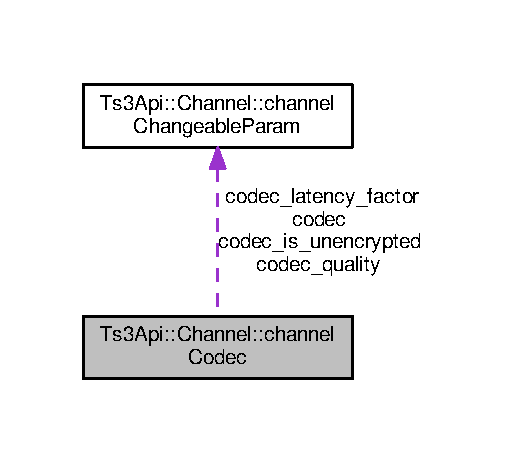
\includegraphics[width=243pt]{struct_ts3_api_1_1_channel_1_1channel_codec__coll__graph}
\end{center}
\end{figure}
\subsection*{Public Attributes}
\begin{DoxyCompactItemize}
\item 
\hyperlink{struct_ts3_api_1_1_channel_1_1channel_changeable_param}{channel\+Changeable\+Param} {\bfseries codec} = \hyperlink{struct_ts3_api_1_1_channel_1_1channel_changeable_param}{channel\+Changeable\+Param}(N\+U\+LL, \char`\"{}channel\+\_\+codec\char`\"{})\hypertarget{struct_ts3_api_1_1_channel_1_1channel_codec_ab00b6caa9fa7d81f62d9044eb0d81e39}{}\label{struct_ts3_api_1_1_channel_1_1channel_codec_ab00b6caa9fa7d81f62d9044eb0d81e39}

\item 
\hyperlink{struct_ts3_api_1_1_channel_1_1channel_changeable_param}{channel\+Changeable\+Param} {\bfseries codec\+\_\+quality} = \hyperlink{struct_ts3_api_1_1_channel_1_1channel_changeable_param}{channel\+Changeable\+Param}(N\+U\+LL, \char`\"{}channel\+\_\+codec\+\_\+quality\char`\"{})\hypertarget{struct_ts3_api_1_1_channel_1_1channel_codec_a17025f34997a4e3c066dfdbea686b02d}{}\label{struct_ts3_api_1_1_channel_1_1channel_codec_a17025f34997a4e3c066dfdbea686b02d}

\item 
\hyperlink{struct_ts3_api_1_1_channel_1_1channel_changeable_param}{channel\+Changeable\+Param} {\bfseries codec\+\_\+latency\+\_\+factor} = \hyperlink{struct_ts3_api_1_1_channel_1_1channel_changeable_param}{channel\+Changeable\+Param}(N\+U\+LL, \char`\"{}channel\+\_\+codec\+\_\+latency\+\_\+factor\char`\"{})\hypertarget{struct_ts3_api_1_1_channel_1_1channel_codec_a000ada6b4d5ff3c7c3ad593dd3c14828}{}\label{struct_ts3_api_1_1_channel_1_1channel_codec_a000ada6b4d5ff3c7c3ad593dd3c14828}

\item 
\hyperlink{struct_ts3_api_1_1_channel_1_1channel_changeable_param}{channel\+Changeable\+Param} {\bfseries codec\+\_\+is\+\_\+unencrypted} = \hyperlink{struct_ts3_api_1_1_channel_1_1channel_changeable_param}{channel\+Changeable\+Param}(N\+U\+LL, \char`\"{}channel\+\_\+codec\+\_\+is\+\_\+unencrypted\char`\"{})\hypertarget{struct_ts3_api_1_1_channel_1_1channel_codec_aea7986a0df5f717e4da96dad5768a860}{}\label{struct_ts3_api_1_1_channel_1_1channel_codec_aea7986a0df5f717e4da96dad5768a860}

\end{DoxyCompactItemize}


\subsection{Detailed Description}
Contain channel codec settings. 

The documentation for this struct was generated from the following file\+:\begin{DoxyCompactItemize}
\item 
/home/karol/projects/\+Team\+Speak3-\/\+C-\/\+Query-\/\+A\+P\+I/src/includes/Channel.\+hpp\end{DoxyCompactItemize}

\hypertarget{struct_ts3_api_1_1_channel_1_1channel_flags}{}\section{Ts3\+Api\+:\+:Channel\+:\+:channel\+Flags Struct Reference}
\label{struct_ts3_api_1_1_channel_1_1channel_flags}\index{Ts3\+Api\+::\+Channel\+::channel\+Flags@{Ts3\+Api\+::\+Channel\+::channel\+Flags}}


Contain channel flags.  




{\ttfamily \#include $<$Channel.\+hpp$>$}



Collaboration diagram for Ts3\+Api\+:\+:Channel\+:\+:channel\+Flags\+:\nopagebreak
\begin{figure}[H]
\begin{center}
\leavevmode
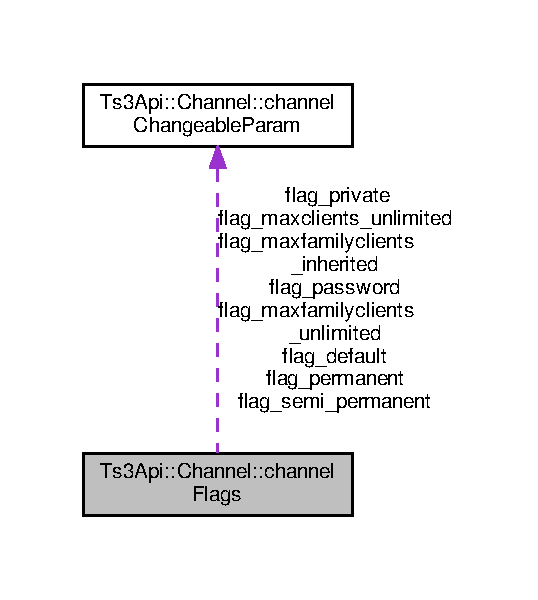
\includegraphics[width=258pt]{struct_ts3_api_1_1_channel_1_1channel_flags__coll__graph}
\end{center}
\end{figure}
\subsection*{Public Attributes}
\begin{DoxyCompactItemize}
\item 
\hyperlink{struct_ts3_api_1_1_channel_1_1channel_changeable_param}{channel\+Changeable\+Param} {\bfseries flag\+\_\+permanent} = \hyperlink{struct_ts3_api_1_1_channel_1_1channel_changeable_param}{channel\+Changeable\+Param}(N\+U\+LL, \char`\"{}channel\+\_\+flag\+\_\+permanent\char`\"{})\hypertarget{struct_ts3_api_1_1_channel_1_1channel_flags_a30f06e347962f1d6ac2d50a4bee87bd1}{}\label{struct_ts3_api_1_1_channel_1_1channel_flags_a30f06e347962f1d6ac2d50a4bee87bd1}

\item 
\hyperlink{struct_ts3_api_1_1_channel_1_1channel_changeable_param}{channel\+Changeable\+Param} {\bfseries flag\+\_\+semi\+\_\+permanent} = \hyperlink{struct_ts3_api_1_1_channel_1_1channel_changeable_param}{channel\+Changeable\+Param}(N\+U\+LL, \char`\"{}channel\+\_\+flag\+\_\+semi\+\_\+permanent\char`\"{})\hypertarget{struct_ts3_api_1_1_channel_1_1channel_flags_a6b92e7212b84b51adcd92db79e21a425}{}\label{struct_ts3_api_1_1_channel_1_1channel_flags_a6b92e7212b84b51adcd92db79e21a425}

\item 
\hyperlink{struct_ts3_api_1_1_channel_1_1channel_changeable_param}{channel\+Changeable\+Param} {\bfseries flag\+\_\+default} = \hyperlink{struct_ts3_api_1_1_channel_1_1channel_changeable_param}{channel\+Changeable\+Param}(N\+U\+LL, \char`\"{}channel\+\_\+flag\+\_\+default\char`\"{})\hypertarget{struct_ts3_api_1_1_channel_1_1channel_flags_a875dce3e91976886ee4c45574a2389a5}{}\label{struct_ts3_api_1_1_channel_1_1channel_flags_a875dce3e91976886ee4c45574a2389a5}

\item 
\hyperlink{struct_ts3_api_1_1_channel_1_1channel_changeable_param}{channel\+Changeable\+Param} {\bfseries flag\+\_\+password} = \hyperlink{struct_ts3_api_1_1_channel_1_1channel_changeable_param}{channel\+Changeable\+Param}(N\+U\+LL, \char`\"{}channel\+\_\+flag\+\_\+password\char`\"{})\hypertarget{struct_ts3_api_1_1_channel_1_1channel_flags_a5dcf754a6f091d86d62d0781c8c6b1ed}{}\label{struct_ts3_api_1_1_channel_1_1channel_flags_a5dcf754a6f091d86d62d0781c8c6b1ed}

\item 
\hyperlink{struct_ts3_api_1_1_channel_1_1channel_changeable_param}{channel\+Changeable\+Param} {\bfseries flag\+\_\+maxclients\+\_\+unlimited} = \hyperlink{struct_ts3_api_1_1_channel_1_1channel_changeable_param}{channel\+Changeable\+Param}(N\+U\+LL, \char`\"{}channel\+\_\+flag\+\_\+maxclients\+\_\+unlimited\char`\"{})\hypertarget{struct_ts3_api_1_1_channel_1_1channel_flags_ae26808390709dbf4ef3be039abe20669}{}\label{struct_ts3_api_1_1_channel_1_1channel_flags_ae26808390709dbf4ef3be039abe20669}

\item 
\hyperlink{struct_ts3_api_1_1_channel_1_1channel_changeable_param}{channel\+Changeable\+Param} {\bfseries flag\+\_\+maxfamilyclients\+\_\+unlimited} = \hyperlink{struct_ts3_api_1_1_channel_1_1channel_changeable_param}{channel\+Changeable\+Param}(N\+U\+LL, \char`\"{}channel\+\_\+flag\+\_\+maxfamilyclients\+\_\+unlimited\char`\"{})\hypertarget{struct_ts3_api_1_1_channel_1_1channel_flags_a4c7b3a5415749ae58828b1c4cbeddedd}{}\label{struct_ts3_api_1_1_channel_1_1channel_flags_a4c7b3a5415749ae58828b1c4cbeddedd}

\item 
\hyperlink{struct_ts3_api_1_1_channel_1_1channel_changeable_param}{channel\+Changeable\+Param} {\bfseries flag\+\_\+maxfamilyclients\+\_\+inherited} = \hyperlink{struct_ts3_api_1_1_channel_1_1channel_changeable_param}{channel\+Changeable\+Param}(N\+U\+LL, \char`\"{}channel\+\_\+flag\+\_\+maxfamilyclients\+\_\+inherited\char`\"{})\hypertarget{struct_ts3_api_1_1_channel_1_1channel_flags_aff6c5c0b0bc8a01ebc33066a93d5d237}{}\label{struct_ts3_api_1_1_channel_1_1channel_flags_aff6c5c0b0bc8a01ebc33066a93d5d237}

\item 
\hyperlink{struct_ts3_api_1_1_channel_1_1channel_changeable_param}{channel\+Changeable\+Param} {\bfseries flag\+\_\+private} = \hyperlink{struct_ts3_api_1_1_channel_1_1channel_changeable_param}{channel\+Changeable\+Param}(N\+U\+LL, \char`\"{}channel\+\_\+flag\+\_\+private\char`\"{})\hypertarget{struct_ts3_api_1_1_channel_1_1channel_flags_a2c3f5277269123eb04e11a03aafe9937}{}\label{struct_ts3_api_1_1_channel_1_1channel_flags_a2c3f5277269123eb04e11a03aafe9937}

\end{DoxyCompactItemize}


\subsection{Detailed Description}
Contain channel flags. 

The documentation for this struct was generated from the following file\+:\begin{DoxyCompactItemize}
\item 
/home/karol/projects/\+Team\+Speak3-\/\+C-\/\+Query-\/\+A\+P\+I/src/includes/Channel.\+hpp\end{DoxyCompactItemize}

\hypertarget{struct_ts3_api_1_1_channel_1_1channel_name}{}\section{Ts3\+Api\+:\+:Channel\+:\+:channel\+Name Struct Reference}
\label{struct_ts3_api_1_1_channel_1_1channel_name}\index{Ts3\+Api\+::\+Channel\+::channel\+Name@{Ts3\+Api\+::\+Channel\+::channel\+Name}}


Contain channel names.  




{\ttfamily \#include $<$Channel.\+hpp$>$}



Collaboration diagram for Ts3\+Api\+:\+:Channel\+:\+:channel\+Name\+:\nopagebreak
\begin{figure}[H]
\begin{center}
\leavevmode
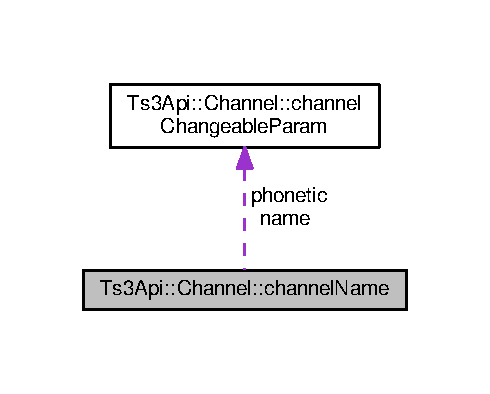
\includegraphics[width=235pt]{struct_ts3_api_1_1_channel_1_1channel_name__coll__graph}
\end{center}
\end{figure}
\subsection*{Public Attributes}
\begin{DoxyCompactItemize}
\item 
\hyperlink{struct_ts3_api_1_1_channel_1_1channel_changeable_param}{channel\+Changeable\+Param} {\bfseries name} = \hyperlink{struct_ts3_api_1_1_channel_1_1channel_changeable_param}{channel\+Changeable\+Param}(N\+U\+LL, \char`\"{}channel\+\_\+name\char`\"{})\hypertarget{struct_ts3_api_1_1_channel_1_1channel_name_af32e3a8d14c7751cd56457792f4833ac}{}\label{struct_ts3_api_1_1_channel_1_1channel_name_af32e3a8d14c7751cd56457792f4833ac}

\item 
\hyperlink{struct_ts3_api_1_1_channel_1_1channel_changeable_param}{channel\+Changeable\+Param} {\bfseries phonetic} = \hyperlink{struct_ts3_api_1_1_channel_1_1channel_changeable_param}{channel\+Changeable\+Param}(N\+U\+LL, \char`\"{}channel\+\_\+name\+\_\+phonetic\char`\"{})\hypertarget{struct_ts3_api_1_1_channel_1_1channel_name_a8e4cfbfed9c1481bddfd5cb1a69b44d0}{}\label{struct_ts3_api_1_1_channel_1_1channel_name_a8e4cfbfed9c1481bddfd5cb1a69b44d0}

\end{DoxyCompactItemize}


\subsection{Detailed Description}
Contain channel names. 

The documentation for this struct was generated from the following file\+:\begin{DoxyCompactItemize}
\item 
/home/karol/projects/\+Team\+Speak3-\/\+C-\/\+Query-\/\+A\+P\+I/src/includes/Channel.\+hpp\end{DoxyCompactItemize}

\hypertarget{class_ts3_api_1_1_client}{}\section{Dokumentacja klasy Ts3\+Api\+:\+:Client}
\label{class_ts3_api_1_1_client}\index{Ts3\+Api\+::\+Client@{Ts3\+Api\+::\+Client}}
\subsection*{Komponenty}
\begin{DoxyCompactItemize}
\item 
struct \hyperlink{struct_ts3_api_1_1_client_1_1changeable_param}{changeable\+Param}
\item 
struct \hyperlink{struct_ts3_api_1_1_client_1_1client_info_properties}{client\+Info\+Properties}
\item 
struct \hyperlink{struct_ts3_api_1_1_client_1_1connection_info}{connection\+Info}
\item 
struct \hyperlink{struct_ts3_api_1_1_client_1_1_i_ds}{I\+Ds}
\item 
struct \hyperlink{struct_ts3_api_1_1_client_1_1nickname}{nickname}
\item 
struct \hyperlink{struct_ts3_api_1_1_client_1_1properties}{properties}
\item 
struct \hyperlink{struct_ts3_api_1_1_client_1_1property}{property}
\item 
struct \hyperlink{struct_ts3_api_1_1_client_1_1transfer_info}{transfer\+Info}
\end{DoxyCompactItemize}
\subsection*{Metody publiczne}
\begin{DoxyCompactItemize}
\item 
{\bfseries Client} (\hyperlink{class_ts3_api_1_1_server}{Server} \&server, \hyperlink{struct_ts3_api_1_1_client_1_1_i_ds}{I\+Ds} client\+I\+Ds, bool client\+List\+Init=false)\hypertarget{class_ts3_api_1_1_client_ad63f5acca38e884294bdf24883fac068}{}\label{class_ts3_api_1_1_client_ad63f5acca38e884294bdf24883fac068}

\item 
void {\bfseries update} ()\hypertarget{class_ts3_api_1_1_client_a6e7a5e19c40bef39ae1c0f5996b8c471}{}\label{class_ts3_api_1_1_client_a6e7a5e19c40bef39ae1c0f5996b8c471}

\item 
bool {\bfseries good} ()\hypertarget{class_ts3_api_1_1_client_a52f9b3ce0e014563b757afdd6fff4628}{}\label{class_ts3_api_1_1_client_a52f9b3ce0e014563b757afdd6fff4628}

\item 
\hyperlink{struct_ts3_api_1_1_client_1_1property}{property} {\bfseries get\+C\+L\+ID} ()\hypertarget{class_ts3_api_1_1_client_a72d6480e7f921ce9694dffeadab1b79a}{}\label{class_ts3_api_1_1_client_a72d6480e7f921ce9694dffeadab1b79a}

\item 
\hyperlink{struct_ts3_api_1_1_client_1_1property}{property} {\bfseries get\+U\+ID} ()\hypertarget{class_ts3_api_1_1_client_a4f145da31772f851628c0a87042c2942}{}\label{class_ts3_api_1_1_client_a4f145da31772f851628c0a87042c2942}

\item 
\hyperlink{struct_ts3_api_1_1_client_1_1property}{property} {\bfseries get\+D\+B\+ID} ()\hypertarget{class_ts3_api_1_1_client_a3854f5517090c0e8428b2de31aac878a}{}\label{class_ts3_api_1_1_client_a3854f5517090c0e8428b2de31aac878a}

\item 
\hyperlink{struct_ts3_api_1_1_client_1_1property}{property} {\bfseries get\+Idle\+Time} ()\hypertarget{class_ts3_api_1_1_client_a9e72f2d9a120491bb17e8b0871339852}{}\label{class_ts3_api_1_1_client_a9e72f2d9a120491bb17e8b0871339852}

\item 
\hyperlink{struct_ts3_api_1_1_client_1_1nickname}{nickname} {\bfseries get\+Nickname} ()\hypertarget{class_ts3_api_1_1_client_ab4ee104edd30af8926b01cc412c37c77}{}\label{class_ts3_api_1_1_client_ab4ee104edd30af8926b01cc412c37c77}

\item 
\hyperlink{struct_ts3_api_1_1_client_1_1property}{property} {\bfseries get\+Version} ()\hypertarget{class_ts3_api_1_1_client_a1f93d8d831cc99fab88097bd6aef82d6}{}\label{class_ts3_api_1_1_client_a1f93d8d831cc99fab88097bd6aef82d6}

\item 
\hyperlink{struct_ts3_api_1_1_client_1_1property}{property} {\bfseries get\+Version\+Sign} ()\hypertarget{class_ts3_api_1_1_client_a99b8daa6d6d57b878f9a13cd5c9e0af5}{}\label{class_ts3_api_1_1_client_a99b8daa6d6d57b878f9a13cd5c9e0af5}

\item 
\hyperlink{struct_ts3_api_1_1_client_1_1property}{property} {\bfseries get\+Platform} ()\hypertarget{class_ts3_api_1_1_client_ae99c8f0daeea7427a58ed2f9169371b8}{}\label{class_ts3_api_1_1_client_ae99c8f0daeea7427a58ed2f9169371b8}

\item 
bool {\bfseries get\+Input\+Muted} ()\hypertarget{class_ts3_api_1_1_client_aea54e6f6b4678970b4ea40e4a6e6c162}{}\label{class_ts3_api_1_1_client_aea54e6f6b4678970b4ea40e4a6e6c162}

\item 
bool {\bfseries get\+Output\+Muted} ()\hypertarget{class_ts3_api_1_1_client_a474beabfe41f4e41a4e4b6792e6c5091}{}\label{class_ts3_api_1_1_client_a474beabfe41f4e41a4e4b6792e6c5091}

\item 
bool {\bfseries get\+Output\+Only\+Muted} ()\hypertarget{class_ts3_api_1_1_client_a859e0e44c5d088d5e170ab537f6e095d}{}\label{class_ts3_api_1_1_client_a859e0e44c5d088d5e170ab537f6e095d}

\item 
bool {\bfseries get\+Input\+Hardware} ()\hypertarget{class_ts3_api_1_1_client_a5f4d9189c98341b0bd0559d3a2f246a5}{}\label{class_ts3_api_1_1_client_a5f4d9189c98341b0bd0559d3a2f246a5}

\item 
bool {\bfseries get\+Output\+Hardware} ()\hypertarget{class_ts3_api_1_1_client_a7ade8fb756646429b0a76c021c8beb45}{}\label{class_ts3_api_1_1_client_a7ade8fb756646429b0a76c021c8beb45}

\item 
\hyperlink{struct_ts3_api_1_1_client_1_1property}{property} {\bfseries get\+Default\+Channel} ()\hypertarget{class_ts3_api_1_1_client_a47e3ed0dd865ddf3961b90d635d0b941}{}\label{class_ts3_api_1_1_client_a47e3ed0dd865ddf3961b90d635d0b941}

\item 
\hyperlink{struct_ts3_api_1_1_client_1_1property}{property} {\bfseries get\+Meta\+Data} ()\hypertarget{class_ts3_api_1_1_client_abb4417973cacce23cab180e28d0e458e}{}\label{class_ts3_api_1_1_client_abb4417973cacce23cab180e28d0e458e}

\item 
bool {\bfseries get\+Recording\+Status} ()\hypertarget{class_ts3_api_1_1_client_a49bf224894390bb80361fabd2b477be9}{}\label{class_ts3_api_1_1_client_a49bf224894390bb80361fabd2b477be9}

\item 
\hyperlink{struct_ts3_api_1_1_client_1_1property}{property} {\bfseries get\+Security\+Hash} ()\hypertarget{class_ts3_api_1_1_client_ac4dc5825d75d73d9c10ef24caa15484f}{}\label{class_ts3_api_1_1_client_ac4dc5825d75d73d9c10ef24caa15484f}

\item 
\hyperlink{struct_ts3_api_1_1_client_1_1property}{property} {\bfseries get\+Login\+Name} ()\hypertarget{class_ts3_api_1_1_client_a83def7db779ad53a69b47166a85db2c1}{}\label{class_ts3_api_1_1_client_a83def7db779ad53a69b47166a85db2c1}

\item 
\hyperlink{class_ts3_api_1_1_group}{Group} {\bfseries get\+Channel\+Group} ()\hypertarget{class_ts3_api_1_1_client_a55c6f2dc787130636f99cd1c38d65137}{}\label{class_ts3_api_1_1_client_a55c6f2dc787130636f99cd1c38d65137}

\item 
\hyperlink{struct_ts3_api_1_1_client_1_1property}{property} {\bfseries get\+Channel\+Group\+ID} ()\hypertarget{class_ts3_api_1_1_client_aa53d97dbbff17a0e19194d6e5cca8fac}{}\label{class_ts3_api_1_1_client_aa53d97dbbff17a0e19194d6e5cca8fac}

\item 
vector$<$ \hyperlink{class_ts3_api_1_1_group}{Group} $>$ {\bfseries get\+Server\+Groups} ()\hypertarget{class_ts3_api_1_1_client_a0cda9e0c7e285f4936807a7792937c74}{}\label{class_ts3_api_1_1_client_a0cda9e0c7e285f4936807a7792937c74}

\item 
vector$<$ string $>$ {\bfseries get\+Server\+Groups\+List} ()\hypertarget{class_ts3_api_1_1_client_a3b0a069fc62a1ef9e7cad04617da2c96}{}\label{class_ts3_api_1_1_client_a3b0a069fc62a1ef9e7cad04617da2c96}

\item 
\hyperlink{struct_ts3_api_1_1timestamp_time}{timestamp\+Time} {\bfseries get\+Created\+Time} ()\hypertarget{class_ts3_api_1_1_client_a2c003687aa56e5869a825de386934d66}{}\label{class_ts3_api_1_1_client_a2c003687aa56e5869a825de386934d66}

\item 
\hyperlink{struct_ts3_api_1_1timestamp_time}{timestamp\+Time} {\bfseries get\+Lastconnected\+Time} ()\hypertarget{class_ts3_api_1_1_client_a3c7b2b662a6ca58c5d64061310948916}{}\label{class_ts3_api_1_1_client_a3c7b2b662a6ca58c5d64061310948916}

\item 
\hyperlink{struct_ts3_api_1_1_client_1_1property}{property} {\bfseries get\+Total\+Connections} ()\hypertarget{class_ts3_api_1_1_client_a585be182f993f8fef6b3f84eb9a61d49}{}\label{class_ts3_api_1_1_client_a585be182f993f8fef6b3f84eb9a61d49}

\item 
bool {\bfseries get\+Away\+Status} ()\hypertarget{class_ts3_api_1_1_client_a7e92b3d2dd2192570eb593e9eeabb824}{}\label{class_ts3_api_1_1_client_a7e92b3d2dd2192570eb593e9eeabb824}

\item 
\hyperlink{struct_ts3_api_1_1_client_1_1property}{property} {\bfseries get\+Away\+Message} ()\hypertarget{class_ts3_api_1_1_client_a7a9ed475fe2ce1cd1bd13df2b2670a85}{}\label{class_ts3_api_1_1_client_a7a9ed475fe2ce1cd1bd13df2b2670a85}

\item 
\hyperlink{struct_ts3_api_1_1_client_1_1property}{property} {\bfseries get\+Type} ()\hypertarget{class_ts3_api_1_1_client_a0f450e97a7df845fecd966e884e801b7}{}\label{class_ts3_api_1_1_client_a0f450e97a7df845fecd966e884e801b7}

\item 
\hyperlink{struct_ts3_api_1_1_client_1_1property}{property} {\bfseries get\+Avatar\+Flag} ()\hypertarget{class_ts3_api_1_1_client_ad497e8e5075353277cb1592546ac38cf}{}\label{class_ts3_api_1_1_client_ad497e8e5075353277cb1592546ac38cf}

\item 
\hyperlink{class_ts3_api_1_1_permission}{Permission} {\bfseries get\+Talk\+Power} ()\hypertarget{class_ts3_api_1_1_client_a8a88e7e7271f59531d2ad243a8a1ca98}{}\label{class_ts3_api_1_1_client_a8a88e7e7271f59531d2ad243a8a1ca98}

\item 
\hyperlink{struct_ts3_api_1_1_client_1_1property}{property} {\bfseries get\+Talk\+Request} ()\hypertarget{class_ts3_api_1_1_client_a61622917f5ad079cd7c3fde0fd2c488c}{}\label{class_ts3_api_1_1_client_a61622917f5ad079cd7c3fde0fd2c488c}

\item 
\hyperlink{struct_ts3_api_1_1_client_1_1property}{property} {\bfseries get\+Talk\+Request\+Msg} ()\hypertarget{class_ts3_api_1_1_client_a1abf8ffacf99cb032eea2799c810b44e}{}\label{class_ts3_api_1_1_client_a1abf8ffacf99cb032eea2799c810b44e}

\item 
\hyperlink{struct_ts3_api_1_1_client_1_1changeable_param}{changeable\+Param} {\bfseries get\+Description} ()\hypertarget{class_ts3_api_1_1_client_ab322f2946d48e0b72859fc6f22a5a2ec}{}\label{class_ts3_api_1_1_client_ab322f2946d48e0b72859fc6f22a5a2ec}

\item 
\hyperlink{struct_ts3_api_1_1_client_1_1changeable_param}{changeable\+Param} {\bfseries get\+Talker\+Status} ()\hypertarget{class_ts3_api_1_1_client_a8b7a2e220539c7eea441359aa2ec14c0}{}\label{class_ts3_api_1_1_client_a8b7a2e220539c7eea441359aa2ec14c0}

\item 
\hyperlink{struct_ts3_api_1_1_client_1_1transfer_info}{transfer\+Info} {\bfseries get\+Transfer\+Info} ()\hypertarget{class_ts3_api_1_1_client_afa60522220af3207174bd8133c8aab86}{}\label{class_ts3_api_1_1_client_afa60522220af3207174bd8133c8aab86}

\item 
bool {\bfseries get\+Priority\+Speaker\+Status} ()\hypertarget{class_ts3_api_1_1_client_a2b06a02dc27f44f92d75e28eb6e66ddc}{}\label{class_ts3_api_1_1_client_a2b06a02dc27f44f92d75e28eb6e66ddc}

\item 
\hyperlink{class_ts3_api_1_1_permission}{Permission} {\bfseries get\+Needed\+Serverquery\+View\+Power} ()\hypertarget{class_ts3_api_1_1_client_a823273f1c8c4b858b2b416a645e9c245}{}\label{class_ts3_api_1_1_client_a823273f1c8c4b858b2b416a645e9c245}

\item 
\hyperlink{struct_ts3_api_1_1_client_1_1property}{property} {\bfseries get\+Default\+Token} ()\hypertarget{class_ts3_api_1_1_client_ae732cc011b882c77350de6ce99fbd3a0}{}\label{class_ts3_api_1_1_client_ae732cc011b882c77350de6ce99fbd3a0}

\item 
\hyperlink{struct_ts3_api_1_1_client_1_1changeable_param}{changeable\+Param} {\bfseries get\+Icon\+Id} ()\hypertarget{class_ts3_api_1_1_client_a130b1601b40d9e2062d767aa6c68c42d}{}\label{class_ts3_api_1_1_client_a130b1601b40d9e2062d767aa6c68c42d}

\item 
\hyperlink{struct_ts3_api_1_1_client_1_1changeable_param}{changeable\+Param} {\bfseries get\+Channel\+Commander\+Status} ()\hypertarget{class_ts3_api_1_1_client_a6387e63b888385926fee0c8c98fbdbde}{}\label{class_ts3_api_1_1_client_a6387e63b888385926fee0c8c98fbdbde}

\item 
\hyperlink{struct_ts3_api_1_1_client_1_1property}{property} \hyperlink{class_ts3_api_1_1_client_a7aea0d7be0c13772bf0cbcfe435d5b35}{get\+Country} ()
\begin{DoxyCompactList}\small\item\em Zwraca kraj użytkownika. \end{DoxyCompactList}\item 
\hyperlink{struct_ts3_api_1_1_client_1_1property}{property} {\bfseries get\+Channel\+Group\+Inherit\+Channel\+ID} ()\hypertarget{class_ts3_api_1_1_client_a7ca8f8068c190499d056c49496cdb2e8}{}\label{class_ts3_api_1_1_client_a7ca8f8068c190499d056c49496cdb2e8}

\item 
\hyperlink{struct_ts3_api_1_1_client_1_1property}{property} {\bfseries get\+Badges} ()\hypertarget{class_ts3_api_1_1_client_a13b167d84730f97ef069395d58bb2b24}{}\label{class_ts3_api_1_1_client_a13b167d84730f97ef069395d58bb2b24}

\item 
\hyperlink{struct_ts3_api_1_1_client_1_1property}{property} {\bfseries get\+Base64\+Hash\+Client\+U\+ID} ()\hypertarget{class_ts3_api_1_1_client_aea48dfe6fed2db31878bfb46093f315d}{}\label{class_ts3_api_1_1_client_aea48dfe6fed2db31878bfb46093f315d}

\item 
\hyperlink{struct_ts3_api_1_1_client_1_1connection_info}{connection\+Info} {\bfseries get\+Connection\+Info} ()\hypertarget{class_ts3_api_1_1_client_a59fb7b7c522625c35a1d1a8e7e125d5a}{}\label{class_ts3_api_1_1_client_a59fb7b7c522625c35a1d1a8e7e125d5a}

\item 
\hyperlink{struct_ts3_api_1_1ts3_response}{ts3\+Response} {\bfseries add\+Group} (string group\+Id)\hypertarget{class_ts3_api_1_1_client_aa750751c286e1455c1d19c939efd4c0b}{}\label{class_ts3_api_1_1_client_aa750751c286e1455c1d19c939efd4c0b}

\item 
\hyperlink{struct_ts3_api_1_1ts3_response}{ts3\+Response} {\bfseries add\+Group} (const \hyperlink{class_ts3_api_1_1_group}{Group} \&group)\hypertarget{class_ts3_api_1_1_client_a35a6a7ad28623a19bdbb186f871a670c}{}\label{class_ts3_api_1_1_client_a35a6a7ad28623a19bdbb186f871a670c}

\item 
\hyperlink{struct_ts3_api_1_1ts3_response}{ts3\+Response} {\bfseries remove\+Group} (string group\+Id)\hypertarget{class_ts3_api_1_1_client_a8e204f17ea4fc85f7f7c0ffb2da656c2}{}\label{class_ts3_api_1_1_client_a8e204f17ea4fc85f7f7c0ffb2da656c2}

\item 
\hyperlink{struct_ts3_api_1_1ts3_response}{ts3\+Response} {\bfseries remove\+Group} (const \hyperlink{class_ts3_api_1_1_group}{Group} \&group)\hypertarget{class_ts3_api_1_1_client_a7bce985b603efcf0ff8962fcab3a5561}{}\label{class_ts3_api_1_1_client_a7bce985b603efcf0ff8962fcab3a5561}

\item 
\hyperlink{struct_ts3_api_1_1ts3_response}{ts3\+Response} {\bfseries add\+Channel\+Group} (string group\+Id, string channel\+Id)\hypertarget{class_ts3_api_1_1_client_ac98aa52e4c9a76e65f5786ce8197c712}{}\label{class_ts3_api_1_1_client_ac98aa52e4c9a76e65f5786ce8197c712}

\item 
\hyperlink{struct_ts3_api_1_1ts3_response}{ts3\+Response} {\bfseries add\+Channel\+Group} (string group\+Id, const \hyperlink{class_ts3_api_1_1_channel}{Channel} \&channel)\hypertarget{class_ts3_api_1_1_client_aa50ad14f4af3336dc852dd7d836db88f}{}\label{class_ts3_api_1_1_client_aa50ad14f4af3336dc852dd7d836db88f}

\item 
\hyperlink{struct_ts3_api_1_1ts3_response}{ts3\+Response} {\bfseries add\+Channel\+Group} (const \hyperlink{class_ts3_api_1_1_group}{Group} \&group, const \hyperlink{class_ts3_api_1_1_channel}{Channel} \&channel)\hypertarget{class_ts3_api_1_1_client_a4ebbfa0837f4c5d70d40fda76042178d}{}\label{class_ts3_api_1_1_client_a4ebbfa0837f4c5d70d40fda76042178d}

\item 
\hyperlink{struct_ts3_api_1_1ts3_response}{ts3\+Response} {\bfseries add\+Channel\+Group} (const \hyperlink{class_ts3_api_1_1_group}{Group} \&group, string channel\+Id)\hypertarget{class_ts3_api_1_1_client_ae504b68d7d3e8fe32b568e54868392b5}{}\label{class_ts3_api_1_1_client_ae504b68d7d3e8fe32b568e54868392b5}

\item 
\hyperlink{class_ts3_api_1_1_permission}{Permission} {\bfseries get\+Permission} (string perm\+Name)\hypertarget{class_ts3_api_1_1_client_a707da8b57b1d8cea387d740507878170}{}\label{class_ts3_api_1_1_client_a707da8b57b1d8cea387d740507878170}

\item 
\hyperlink{struct_ts3_api_1_1ts3_response}{ts3\+Response} {\bfseries db\+Delete} ()\hypertarget{class_ts3_api_1_1_client_a121f505bf3d9b852c22ee668d6734b3a}{}\label{class_ts3_api_1_1_client_a121f505bf3d9b852c22ee668d6734b3a}

\item 
\hyperlink{struct_ts3_api_1_1ts3_response}{ts3\+Response} {\bfseries set\+Serverquery\+Login} (string login\+Name, string \&password)\hypertarget{class_ts3_api_1_1_client_a277e3458db8f632503f42b3d11d7bf28}{}\label{class_ts3_api_1_1_client_a277e3458db8f632503f42b3d11d7bf28}

\item 
\hyperlink{struct_ts3_api_1_1ts3_response}{ts3\+Response} {\bfseries move} (string cid, string password=\char`\"{}\char`\"{})\hypertarget{class_ts3_api_1_1_client_a1673758a952af1d35e8e7cd1ee2797e7}{}\label{class_ts3_api_1_1_client_a1673758a952af1d35e8e7cd1ee2797e7}

\item 
\hyperlink{struct_ts3_api_1_1ts3_response}{ts3\+Response} {\bfseries kick\+From\+Channel} (string reason)\hypertarget{class_ts3_api_1_1_client_ab381622a51f6ae97b1e137bf7ac6a409}{}\label{class_ts3_api_1_1_client_ab381622a51f6ae97b1e137bf7ac6a409}

\item 
\hyperlink{struct_ts3_api_1_1ts3_response}{ts3\+Response} {\bfseries kick\+From\+Server} (string reason)\hypertarget{class_ts3_api_1_1_client_a6e8af904443616a105b1175bf75af0ac}{}\label{class_ts3_api_1_1_client_a6e8af904443616a105b1175bf75af0ac}

\item 
\hyperlink{struct_ts3_api_1_1ts3_response}{ts3\+Response} {\bfseries poke} (string message)\hypertarget{class_ts3_api_1_1_client_ace50488f45a5a3c823d81cad5b472c36}{}\label{class_ts3_api_1_1_client_ace50488f45a5a3c823d81cad5b472c36}

\item 
\hyperlink{struct_ts3_api_1_1ts3_response}{ts3\+Response} {\bfseries complain} (string message)\hypertarget{class_ts3_api_1_1_client_aa906a4990ae4782977fe57a2ac769afa}{}\label{class_ts3_api_1_1_client_aa906a4990ae4782977fe57a2ac769afa}

\item 
\hyperlink{struct_ts3_api_1_1ts3_response}{ts3\+Response} {\bfseries del\+Complain} (string accuser\+Dbid)\hypertarget{class_ts3_api_1_1_client_a99223aa38b6c0ef75539c701b6a62d88}{}\label{class_ts3_api_1_1_client_a99223aa38b6c0ef75539c701b6a62d88}

\item 
\hyperlink{struct_ts3_api_1_1ts3_response}{ts3\+Response} {\bfseries del\+All\+Complains} ()\hypertarget{class_ts3_api_1_1_client_ac068b0295c2f83931cfc353cc42236ec}{}\label{class_ts3_api_1_1_client_ac068b0295c2f83931cfc353cc42236ec}

\item 
\hyperlink{struct_ts3_api_1_1ts3_response}{ts3\+Response} {\bfseries ban} (string ban\+Time=\char`\"{}\char`\"{}, string reason=\char`\"{}\char`\"{})\hypertarget{class_ts3_api_1_1_client_a41e103e4201cade9384d9e2d19f9f1e5}{}\label{class_ts3_api_1_1_client_a41e103e4201cade9384d9e2d19f9f1e5}

\item 
\hyperlink{struct_ts3_api_1_1ts3_response}{ts3\+Response} {\bfseries send\+Message} (string message)\hypertarget{class_ts3_api_1_1_client_a5ca6d7dcf16e56d5984dfd1782deea95}{}\label{class_ts3_api_1_1_client_a5ca6d7dcf16e56d5984dfd1782deea95}

\end{DoxyCompactItemize}
\subsection*{Przyjaciele}
\begin{DoxyCompactItemize}
\item 
class {\bfseries Permission}\hypertarget{class_ts3_api_1_1_client_ad3834bbd6b2c4839e7f69dc4cc1d6ae6}{}\label{class_ts3_api_1_1_client_ad3834bbd6b2c4839e7f69dc4cc1d6ae6}

\end{DoxyCompactItemize}


\subsection{Dokumentacja funkcji składowych}
\index{Ts3\+Api\+::\+Client@{Ts3\+Api\+::\+Client}!get\+Country@{get\+Country}}
\index{get\+Country@{get\+Country}!Ts3\+Api\+::\+Client@{Ts3\+Api\+::\+Client}}
\subsubsection[{\texorpdfstring{get\+Country()}{getCountry()}}]{\setlength{\rightskip}{0pt plus 5cm}{\bf Client\+::property} Client\+::get\+Country (
\begin{DoxyParamCaption}
{}
\end{DoxyParamCaption}
)}\hypertarget{class_ts3_api_1_1_client_a7aea0d7be0c13772bf0cbcfe435d5b35}{}\label{class_ts3_api_1_1_client_a7aea0d7be0c13772bf0cbcfe435d5b35}


Zwraca kraj użytkownika. 

Siema 

Dokumentacja dla tej klasy została wygenerowana z plików\+:\begin{DoxyCompactItemize}
\item 
/home/karol/projects/ts3\+A\+P\+Iv2/src/includes/Client.\+hpp\item 
/home/karol/projects/ts3\+A\+P\+Iv2/src/Client.\+cpp\end{DoxyCompactItemize}

\hypertarget{struct_ts3_api_1_1_client_1_1client_info_properties}{}\section{Ts3\+Api\+:\+:Client\+:\+:client\+Info\+Properties Struct Reference}
\label{struct_ts3_api_1_1_client_1_1client_info_properties}\index{Ts3\+Api\+::\+Client\+::client\+Info\+Properties@{Ts3\+Api\+::\+Client\+::client\+Info\+Properties}}


Struktura zawierająca informacje z polecenia query\+: \char`\"{}clientinfo\char`\"{}.  




{\ttfamily \#include $<$Client.\+hpp$>$}



Inheritance diagram for Ts3\+Api\+:\+:Client\+:\+:client\+Info\+Properties\+:\nopagebreak
\begin{figure}[H]
\begin{center}
\leavevmode
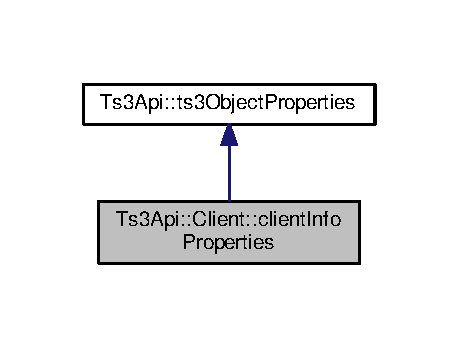
\includegraphics[width=220pt]{struct_ts3_api_1_1_client_1_1client_info_properties__inherit__graph}
\end{center}
\end{figure}


Collaboration diagram for Ts3\+Api\+:\+:Client\+:\+:client\+Info\+Properties\+:\nopagebreak
\begin{figure}[H]
\begin{center}
\leavevmode
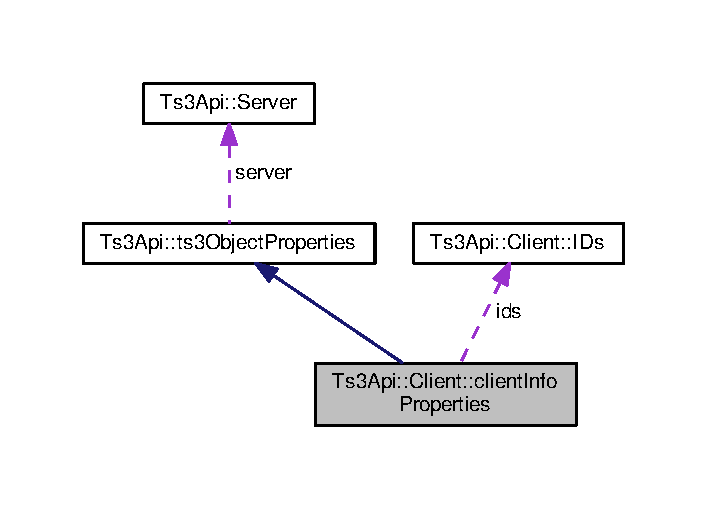
\includegraphics[width=340pt]{struct_ts3_api_1_1_client_1_1client_info_properties__coll__graph}
\end{center}
\end{figure}
\subsection*{Public Member Functions}
\begin{DoxyCompactItemize}
\item 
void {\bfseries update} ()\hypertarget{struct_ts3_api_1_1_client_1_1client_info_properties_a310ed4150a0c315531536fdea3d9105b}{}\label{struct_ts3_api_1_1_client_1_1client_info_properties_a310ed4150a0c315531536fdea3d9105b}

\item 
{\bfseries client\+Info\+Properties} (\hyperlink{struct_ts3_api_1_1_client_1_1_i_ds}{Client\+::\+I\+Ds} \&ids, \hyperlink{class_ts3_api_1_1_server}{Server} \&server, time\+\_\+t \&update\+Time, bool client\+List\+Init)\hypertarget{struct_ts3_api_1_1_client_1_1client_info_properties_ac63f19afca704bfd743863a2069c6608}{}\label{struct_ts3_api_1_1_client_1_1client_info_properties_ac63f19afca704bfd743863a2069c6608}

\end{DoxyCompactItemize}
\subsection*{Public Attributes}
\begin{DoxyCompactItemize}
\item 
\hyperlink{struct_ts3_api_1_1_client_1_1_i_ds}{I\+Ds} \& {\bfseries ids}\hypertarget{struct_ts3_api_1_1_client_1_1client_info_properties_ab52bf97518b969ed50bcb8a0ac9b11da}{}\label{struct_ts3_api_1_1_client_1_1client_info_properties_ab52bf97518b969ed50bcb8a0ac9b11da}

\end{DoxyCompactItemize}
\subsection*{Additional Inherited Members}


\subsection{Detailed Description}
Struktura zawierająca informacje z polecenia query\+: \char`\"{}clientinfo\char`\"{}. 

The documentation for this struct was generated from the following files\+:\begin{DoxyCompactItemize}
\item 
/home/karol/projects/\+Team\+Speak3-\/\+C-\/\+Query-\/\+A\+P\+I/src/includes/Client.\+hpp\item 
/home/karol/projects/\+Team\+Speak3-\/\+C-\/\+Query-\/\+A\+P\+I/src/Client.\+cpp\end{DoxyCompactItemize}

\hypertarget{struct_ts3_api_1_1_client_1_1connection_info}{}\section{Ts3\+Api\+:\+:Client\+:\+:connection\+Info Struct Reference}
\label{struct_ts3_api_1_1_client_1_1connection_info}\index{Ts3\+Api\+::\+Client\+::connection\+Info@{Ts3\+Api\+::\+Client\+::connection\+Info}}


Zawiera informacje o połączeniu danego użykownika.  




{\ttfamily \#include $<$Client.\+hpp$>$}

\subsection*{Public Attributes}
\begin{DoxyCompactItemize}
\item 
string {\bfseries filetransfer\+\_\+bandwidth\+\_\+sent}\hypertarget{struct_ts3_api_1_1_client_1_1connection_info_af83775ea9aa65c99ba6bae8c3b75e311}{}\label{struct_ts3_api_1_1_client_1_1connection_info_af83775ea9aa65c99ba6bae8c3b75e311}

\item 
string {\bfseries filetransfer\+\_\+bandwidth\+\_\+received}\hypertarget{struct_ts3_api_1_1_client_1_1connection_info_aa8cfdea946a89bd88fb57e2833e72497}{}\label{struct_ts3_api_1_1_client_1_1connection_info_aa8cfdea946a89bd88fb57e2833e72497}

\item 
string {\bfseries packets\+\_\+sent\+\_\+total}\hypertarget{struct_ts3_api_1_1_client_1_1connection_info_aa822f6e44c8580a4814dd9dfc9c55ef2}{}\label{struct_ts3_api_1_1_client_1_1connection_info_aa822f6e44c8580a4814dd9dfc9c55ef2}

\item 
string {\bfseries bytes\+\_\+sent\+\_\+total}\hypertarget{struct_ts3_api_1_1_client_1_1connection_info_a6bfc306d8060781261c2aa28b395f5df}{}\label{struct_ts3_api_1_1_client_1_1connection_info_a6bfc306d8060781261c2aa28b395f5df}

\item 
string {\bfseries packets\+\_\+received\+\_\+total}\hypertarget{struct_ts3_api_1_1_client_1_1connection_info_ae6ccbb4cf1cbca10fa890ae86ecc3e29}{}\label{struct_ts3_api_1_1_client_1_1connection_info_ae6ccbb4cf1cbca10fa890ae86ecc3e29}

\item 
string {\bfseries bytes\+\_\+received\+\_\+total}\hypertarget{struct_ts3_api_1_1_client_1_1connection_info_a1448f2fa44e9f33206d6d166f044a718}{}\label{struct_ts3_api_1_1_client_1_1connection_info_a1448f2fa44e9f33206d6d166f044a718}

\item 
string {\bfseries bandwidth\+\_\+sent\+\_\+last\+\_\+second\+\_\+total}\hypertarget{struct_ts3_api_1_1_client_1_1connection_info_afda4313a7d385cf99678ffcc20fe2426}{}\label{struct_ts3_api_1_1_client_1_1connection_info_afda4313a7d385cf99678ffcc20fe2426}

\item 
string {\bfseries bandwidth\+\_\+sent\+\_\+last\+\_\+minute\+\_\+total}\hypertarget{struct_ts3_api_1_1_client_1_1connection_info_a6269b5cc13fd231de2df4be613fe6632}{}\label{struct_ts3_api_1_1_client_1_1connection_info_a6269b5cc13fd231de2df4be613fe6632}

\item 
string {\bfseries bandwidth\+\_\+received\+\_\+last\+\_\+second\+\_\+total}\hypertarget{struct_ts3_api_1_1_client_1_1connection_info_a6d4a4fba176a5934105f604afa6c9c57}{}\label{struct_ts3_api_1_1_client_1_1connection_info_a6d4a4fba176a5934105f604afa6c9c57}

\item 
string {\bfseries bandwidth\+\_\+received\+\_\+last\+\_\+minute\+\_\+total}\hypertarget{struct_ts3_api_1_1_client_1_1connection_info_a3447203e856648cd195d1cc4466cccc1}{}\label{struct_ts3_api_1_1_client_1_1connection_info_a3447203e856648cd195d1cc4466cccc1}

\item 
string {\bfseries connected\+\_\+time}\hypertarget{struct_ts3_api_1_1_client_1_1connection_info_a898099df806c6f2ac4843b1f8cc2a6a1}{}\label{struct_ts3_api_1_1_client_1_1connection_info_a898099df806c6f2ac4843b1f8cc2a6a1}

\item 
string {\bfseries connection\+\_\+client\+\_\+ip}\hypertarget{struct_ts3_api_1_1_client_1_1connection_info_a2b0506154b5a4d7a1c3e4f3dce87b52c}{}\label{struct_ts3_api_1_1_client_1_1connection_info_a2b0506154b5a4d7a1c3e4f3dce87b52c}

\end{DoxyCompactItemize}


\subsection{Detailed Description}
Zawiera informacje o połączeniu danego użykownika. 

The documentation for this struct was generated from the following file\+:\begin{DoxyCompactItemize}
\item 
/home/karol/projects/\+Team\+Speak3-\/\+C-\/\+Query-\/\+A\+P\+I/src/includes/Client.\+hpp\end{DoxyCompactItemize}

\hypertarget{struct_ts3_api_1_1error}{}\section{Ts3\+Api\+:\+:error Struct Reference}
\label{struct_ts3_api_1_1error}\index{Ts3\+Api\+::error@{Ts3\+Api\+::error}}
\subsection*{Public Member Functions}
\begin{DoxyCompactItemize}
\item 
{\bfseries error} (string msg=\char`\"{}\char`\"{}, int id=0)\hypertarget{struct_ts3_api_1_1error_a03255b3eab76cd950fdfb4ec843cbec6}{}\label{struct_ts3_api_1_1error_a03255b3eab76cd950fdfb4ec843cbec6}

\end{DoxyCompactItemize}
\subsection*{Public Attributes}
\begin{DoxyCompactItemize}
\item 
string {\bfseries msg} = \char`\"{}\char`\"{}\hypertarget{struct_ts3_api_1_1error_ac72761d3bd826d444d0d342a27b64f68}{}\label{struct_ts3_api_1_1error_ac72761d3bd826d444d0d342a27b64f68}

\item 
int {\bfseries id} = 0\hypertarget{struct_ts3_api_1_1error_a3c86d7bb5a4db46e71b00c78c482c6b9}{}\label{struct_ts3_api_1_1error_a3c86d7bb5a4db46e71b00c78c482c6b9}

\end{DoxyCompactItemize}


The documentation for this struct was generated from the following files\+:\begin{DoxyCompactItemize}
\item 
/home/karol/projects/\+Team\+Speak3-\/\+C-\/\+Query-\/\+A\+P\+I/src/includes/structs/server\+Structs.\+hpp\item 
/home/karol/projects/\+Team\+Speak3-\/\+C-\/\+Query-\/\+A\+P\+I/src/server\+Structs.\+cpp\end{DoxyCompactItemize}

\hypertarget{class_ts3_api_1_1_group}{}\section{Dokumentacja klasy Ts3\+Api\+:\+:Group}
\label{class_ts3_api_1_1_group}\index{Ts3\+Api\+::\+Group@{Ts3\+Api\+::\+Group}}
\subsection*{Metody publiczne}
\begin{DoxyCompactItemize}
\item 
{\bfseries Group} (\hyperlink{class_ts3_api_1_1_server}{Server} \&server, string id)\hypertarget{class_ts3_api_1_1_group_a13b108d520b74048200fef48eecf0d72}{}\label{class_ts3_api_1_1_group_a13b108d520b74048200fef48eecf0d72}

\end{DoxyCompactItemize}
\subsection*{Przyjaciele}
\begin{DoxyCompactItemize}
\item 
class {\bfseries Client}\hypertarget{class_ts3_api_1_1_group_a5db1c99e2c94b26278f3838c85cdb618}{}\label{class_ts3_api_1_1_group_a5db1c99e2c94b26278f3838c85cdb618}

\item 
class {\bfseries Server}\hypertarget{class_ts3_api_1_1_group_ac2055578ac48afabe5af487878450f68}{}\label{class_ts3_api_1_1_group_ac2055578ac48afabe5af487878450f68}

\item 
class {\bfseries Permission}\hypertarget{class_ts3_api_1_1_group_ad3834bbd6b2c4839e7f69dc4cc1d6ae6}{}\label{class_ts3_api_1_1_group_ad3834bbd6b2c4839e7f69dc4cc1d6ae6}

\end{DoxyCompactItemize}


Dokumentacja dla tej klasy została wygenerowana z plików\+:\begin{DoxyCompactItemize}
\item 
/home/karol/projects/ts3\+A\+P\+Iv2/src/includes/Group.\+hpp\item 
/home/karol/projects/ts3\+A\+P\+Iv2/src/Group.\+cpp\end{DoxyCompactItemize}

\hypertarget{struct_ts3_api_1_1_client_1_1_i_ds}{}\section{Ts3\+Api\+:\+:Client\+:\+:I\+Ds Struct Reference}
\label{struct_ts3_api_1_1_client_1_1_i_ds}\index{Ts3\+Api\+::\+Client\+::\+I\+Ds@{Ts3\+Api\+::\+Client\+::\+I\+Ds}}


Zbiór indentyfikatorów użytkownika.  




{\ttfamily \#include $<$Client.\+hpp$>$}

\subsection*{Public Member Functions}
\begin{DoxyCompactItemize}
\item 
{\bfseries I\+Ds} (string clid=\char`\"{}unknown\char`\"{}, string uid=\char`\"{}unknown\char`\"{}, string dbid=\char`\"{}unknown\char`\"{})\hypertarget{struct_ts3_api_1_1_client_1_1_i_ds_a09b63cd33e2cda211b9602331fcbc479}{}\label{struct_ts3_api_1_1_client_1_1_i_ds_a09b63cd33e2cda211b9602331fcbc479}

\end{DoxyCompactItemize}
\subsection*{Public Attributes}
\begin{DoxyCompactItemize}
\item 
string {\bfseries dbid} = \char`\"{}unknown\char`\"{}\hypertarget{struct_ts3_api_1_1_client_1_1_i_ds_a24bc7b82dce19a9aedbc44cd3962da29}{}\label{struct_ts3_api_1_1_client_1_1_i_ds_a24bc7b82dce19a9aedbc44cd3962da29}

\item 
string {\bfseries clid} = \char`\"{}unknown\char`\"{}\hypertarget{struct_ts3_api_1_1_client_1_1_i_ds_a9629faff180a32d054f11316a5accd0d}{}\label{struct_ts3_api_1_1_client_1_1_i_ds_a9629faff180a32d054f11316a5accd0d}

\item 
string {\bfseries uid} = \char`\"{}unknown\char`\"{}\hypertarget{struct_ts3_api_1_1_client_1_1_i_ds_aea719a541ce3791f6753e3acf25b9b64}{}\label{struct_ts3_api_1_1_client_1_1_i_ds_aea719a541ce3791f6753e3acf25b9b64}

\end{DoxyCompactItemize}


\subsection{Detailed Description}
Zbiór indentyfikatorów użytkownika. 

The documentation for this struct was generated from the following files\+:\begin{DoxyCompactItemize}
\item 
/home/karol/projects/\+Team\+Speak3-\/\+C-\/\+Query-\/\+A\+P\+I/src/includes/Client.\+hpp\item 
/home/karol/projects/\+Team\+Speak3-\/\+C-\/\+Query-\/\+A\+P\+I/src/Client.\+cpp\end{DoxyCompactItemize}

\hypertarget{struct_ts3_api_1_1_client_1_1nickname}{}\section{Ts3\+Api\+:\+:Client\+:\+:nickname Struct Reference}
\label{struct_ts3_api_1_1_client_1_1nickname}\index{Ts3\+Api\+::\+Client\+::nickname@{Ts3\+Api\+::\+Client\+::nickname}}
\subsection*{Public Member Functions}
\begin{DoxyCompactItemize}
\item 
{\bfseries nickname} (string \hyperlink{struct_ts3_api_1_1_client_1_1nickname}{nickname}, string phonetic)\hypertarget{struct_ts3_api_1_1_client_1_1nickname_a1b89520081796e96c17bb041900265bc}{}\label{struct_ts3_api_1_1_client_1_1nickname_a1b89520081796e96c17bb041900265bc}

\end{DoxyCompactItemize}
\subsection*{Public Attributes}
\begin{DoxyCompactItemize}
\item 
string {\bfseries value}\hypertarget{struct_ts3_api_1_1_client_1_1nickname_a0c0b1bd5e3cfc5eb90d0ba98428ef398}{}\label{struct_ts3_api_1_1_client_1_1nickname_a0c0b1bd5e3cfc5eb90d0ba98428ef398}

\item 
string {\bfseries phonetic}\hypertarget{struct_ts3_api_1_1_client_1_1nickname_aa6e3a9190205ddf1cca72c279376b7c4}{}\label{struct_ts3_api_1_1_client_1_1nickname_aa6e3a9190205ddf1cca72c279376b7c4}

\end{DoxyCompactItemize}


The documentation for this struct was generated from the following files\+:\begin{DoxyCompactItemize}
\item 
/home/karol/projects/\+Team\+Speak3-\/\+C-\/\+Query-\/\+A\+P\+I/src/includes/Client.\+hpp\item 
/home/karol/projects/\+Team\+Speak3-\/\+C-\/\+Query-\/\+A\+P\+I/src/Client.\+cpp\end{DoxyCompactItemize}

\hypertarget{class_ts3_api_1_1_permission}{}\section{Ts3\+Api\+:\+:Permission Class Reference}
\label{class_ts3_api_1_1_permission}\index{Ts3\+Api\+::\+Permission@{Ts3\+Api\+::\+Permission}}
\subsection*{Public Types}
\begin{DoxyCompactItemize}
\item 
enum {\bfseries Permission\+Group\+Types} \{ \\*
{\bfseries Perm\+Group\+Type\+Server\+Group} = 0, 
{\bfseries Perm\+Group\+Type\+Global\+Client}, 
{\bfseries Perm\+Group\+Type\+Channel}, 
{\bfseries Perm\+Group\+Type\+Channel\+Group}, 
\\*
{\bfseries Perm\+Group\+Type\+Channel\+Client}
 \}\hypertarget{class_ts3_api_1_1_permission_a9ce809facb0ce3404580d1bd485a0602}{}\label{class_ts3_api_1_1_permission_a9ce809facb0ce3404580d1bd485a0602}

\end{DoxyCompactItemize}
\subsection*{Public Member Functions}
\begin{DoxyCompactItemize}
\item 
{\bfseries Permission} (\hyperlink{class_ts3_api_1_1_client}{Client} \&client, string perm\+Name, string perm\+Value=\char`\"{}unknown\char`\"{})\hypertarget{class_ts3_api_1_1_permission_a23776714b17d9ee0f797d753d2f2fd7c}{}\label{class_ts3_api_1_1_permission_a23776714b17d9ee0f797d753d2f2fd7c}

\item 
{\bfseries Permission} (\hyperlink{class_ts3_api_1_1_channel}{Channel} \&channel, string perm\+Name, string perm\+Value=\char`\"{}unknown\char`\"{})\hypertarget{class_ts3_api_1_1_permission_a5d5631490a405de685e2808b07804634}{}\label{class_ts3_api_1_1_permission_a5d5631490a405de685e2808b07804634}

\item 
{\bfseries Permission} (\hyperlink{class_ts3_api_1_1_group}{Group} \&group, Permission\+Group\+Types perm\+Type, string perm\+Name, string perm\+Value=\char`\"{}unknown\char`\"{})\hypertarget{class_ts3_api_1_1_permission_aca1a5d43dbaed5958de510891b3c222d}{}\label{class_ts3_api_1_1_permission_aca1a5d43dbaed5958de510891b3c222d}

\item 
{\bfseries Permission} (\hyperlink{class_ts3_api_1_1_channel}{Channel} \&channel, \hyperlink{class_ts3_api_1_1_client}{Client} \&client, string perm\+Name, string perm\+Value=\char`\"{}unknown\char`\"{})\hypertarget{class_ts3_api_1_1_permission_a1ef81bfe7b4b293129150c76a675efe6}{}\label{class_ts3_api_1_1_permission_a1ef81bfe7b4b293129150c76a675efe6}

\item 
string {\bfseries get\+Value} ()\hypertarget{class_ts3_api_1_1_permission_a10dfa432a057a22ef4f2564f4246fcad}{}\label{class_ts3_api_1_1_permission_a10dfa432a057a22ef4f2564f4246fcad}

\item 
\hyperlink{struct_ts3_api_1_1ts3_response}{ts3\+Response} {\bfseries update\+Value} ()\hypertarget{class_ts3_api_1_1_permission_a7c3bc67c4c4e8dfe5426b7ff3f7df91a}{}\label{class_ts3_api_1_1_permission_a7c3bc67c4c4e8dfe5426b7ff3f7df91a}

\item 
\hyperlink{struct_ts3_api_1_1ts3_response}{ts3\+Response} {\bfseries new\+Value} (string value, bool perm\+Skip=false, bool perm\+Negated=false)\hypertarget{class_ts3_api_1_1_permission_a8ad645707969516438deb0db0132024e}{}\label{class_ts3_api_1_1_permission_a8ad645707969516438deb0db0132024e}

\item 
\hyperlink{struct_ts3_api_1_1ts3_response}{ts3\+Response} {\bfseries remove} ()\hypertarget{class_ts3_api_1_1_permission_a0afab6f74c467118a231955909012fc2}{}\label{class_ts3_api_1_1_permission_a0afab6f74c467118a231955909012fc2}

\end{DoxyCompactItemize}
\subsection*{Public Attributes}
\begin{DoxyCompactItemize}
\item 
string {\bfseries value}\hypertarget{class_ts3_api_1_1_permission_ae096a38d2f9bb6850ddca16d5d71f71c}{}\label{class_ts3_api_1_1_permission_ae096a38d2f9bb6850ddca16d5d71f71c}

\end{DoxyCompactItemize}
\subsection*{Friends}
\begin{DoxyCompactItemize}
\item 
class {\bfseries Group}\hypertarget{class_ts3_api_1_1_permission_a2697825715974a353728f0d4d5658112}{}\label{class_ts3_api_1_1_permission_a2697825715974a353728f0d4d5658112}

\end{DoxyCompactItemize}


The documentation for this class was generated from the following files\+:\begin{DoxyCompactItemize}
\item 
/home/karol/projects/\+Team\+Speak3-\/\+C-\/\+Query-\/\+A\+P\+I/src/includes/Permission.\+hpp\item 
/home/karol/projects/\+Team\+Speak3-\/\+C-\/\+Query-\/\+A\+P\+I/src/Permission.\+cpp\end{DoxyCompactItemize}

\hypertarget{struct_ts3_api_1_1property}{}\section{Ts3\+Api\+:\+:property Struct Reference}
\label{struct_ts3_api_1_1property}\index{Ts3\+Api\+::property@{Ts3\+Api\+::property}}
\subsection*{Public Member Functions}
\begin{DoxyCompactItemize}
\item 
{\bfseries property} (string name=\char`\"{}unknown\char`\"{}, string value=\char`\"{}unknown\char`\"{})\hypertarget{struct_ts3_api_1_1property_a00b64cf56643cd8e684c7f7d6adb1383}{}\label{struct_ts3_api_1_1property_a00b64cf56643cd8e684c7f7d6adb1383}

\end{DoxyCompactItemize}
\subsection*{Public Attributes}
\begin{DoxyCompactItemize}
\item 
string {\bfseries name}\hypertarget{struct_ts3_api_1_1property_a1264609664cf7b97301c7b5afa57db1b}{}\label{struct_ts3_api_1_1property_a1264609664cf7b97301c7b5afa57db1b}

\item 
string {\bfseries value}\hypertarget{struct_ts3_api_1_1property_ac0864899755720986c7113aa2e35ea7f}{}\label{struct_ts3_api_1_1property_ac0864899755720986c7113aa2e35ea7f}

\end{DoxyCompactItemize}


The documentation for this struct was generated from the following files\+:\begin{DoxyCompactItemize}
\item 
/home/karol/projects/\+Team\+Speak3-\/\+C-\/\+Query-\/\+A\+P\+I/src/includes/structs/ts3\+Object\+Properties.\+hpp\item 
/home/karol/projects/\+Team\+Speak3-\/\+C-\/\+Query-\/\+A\+P\+I/src/ts3\+Object\+Properties.\+cpp\end{DoxyCompactItemize}

\hypertarget{class_ts3_api_1_1_server}{}\section{Ts3\+Api\+:\+:Server Class Reference}
\label{class_ts3_api_1_1_server}\index{Ts3\+Api\+::\+Server@{Ts3\+Api\+::\+Server}}


\hyperlink{class_ts3_api_1_1_server}{Server} Class.  




{\ttfamily \#include $<$Server.\+hpp$>$}

\subsection*{Public Member Functions}
\begin{DoxyCompactItemize}
\item 
\hyperlink{struct_ts3_api_1_1ts3_response}{ts3\+Response} \hyperlink{class_ts3_api_1_1_server_a3ea16dc4a1a611c444c17b0be04d4f45}{execute\+Command} (string command)
\begin{DoxyCompactList}\small\item\em Performs selected command on Ts3 \hyperlink{class_ts3_api_1_1_server}{Server}. \end{DoxyCompactList}\item 
\hyperlink{class_ts3_api_1_1_server_a58ee97b7e2b067978cbcdb8a594687f2}{Server} (string ip, string port)
\begin{DoxyCompactList}\small\item\em Creating and connectiong connection with Ts3\+Server. \end{DoxyCompactList}\item 
\hyperlink{class_ts3_api_1_1_server_a4b3aa2579cb1c8cd1d069582c14d0fa6}{$\sim$\+Server} ()\hypertarget{class_ts3_api_1_1_server_a4b3aa2579cb1c8cd1d069582c14d0fa6}{}\label{class_ts3_api_1_1_server_a4b3aa2579cb1c8cd1d069582c14d0fa6}

\begin{DoxyCompactList}\small\item\em Destroys the object. \end{DoxyCompactList}\item 
bool \hyperlink{class_ts3_api_1_1_server_a947c45de5db2315434a42db1bf024c4c}{connected} ()
\begin{DoxyCompactList}\small\item\em Checks connection with Ts3 \hyperlink{class_ts3_api_1_1_server}{Server}. \end{DoxyCompactList}\item 
\hyperlink{struct_ts3_api_1_1error}{error} \hyperlink{class_ts3_api_1_1_server_aaf8438c60bf85b8859d2f3cf2c0ae394}{get\+Error} ()
\begin{DoxyCompactList}\small\item\em Return last error. \end{DoxyCompactList}\item 
\hyperlink{struct_ts3_api_1_1ts3_response}{ts3\+Response} \hyperlink{class_ts3_api_1_1_server_aa7baa3564ee6d2233f9e9a7f21852b03}{select\+Server} (string port)
\begin{DoxyCompactList}\small\item\em Selects Ts3 server. \end{DoxyCompactList}\item 
\hyperlink{struct_ts3_api_1_1ts3_response}{ts3\+Response} \hyperlink{class_ts3_api_1_1_server_a23702c6673e012c75f5ad884dbc90d4d}{login} (string login, string password)
\begin{DoxyCompactList}\small\item\em Login to Ts3 \hyperlink{class_ts3_api_1_1_server}{Server}. \end{DoxyCompactList}\item 
\hyperlink{class_ts3_api_1_1_client}{Client} \hyperlink{class_ts3_api_1_1_server_a99295e7a116284d1622c7313b3a50977}{get\+Client\+By\+Clid} (string clid)
\begin{DoxyCompactList}\small\item\em Gets the client by clid. \end{DoxyCompactList}\item 
\hyperlink{class_ts3_api_1_1_client}{Client} \hyperlink{class_ts3_api_1_1_server_a29d600f140df9d30158b29ab649c6ec8}{get\+Client\+By\+Dbid} (string dbid)
\begin{DoxyCompactList}\small\item\em Gets the client by dbid. \end{DoxyCompactList}\item 
\hyperlink{class_ts3_api_1_1_client}{Client} \hyperlink{class_ts3_api_1_1_server_aed494922b927ed93491f798c42d4cc37}{get\+Client\+By\+Uid} (string uid)
\begin{DoxyCompactList}\small\item\em Gets the client by uid. \end{DoxyCompactList}\item 
\hyperlink{class_ts3_api_1_1_client}{Client} \hyperlink{class_ts3_api_1_1_server_a235d7e5596be98d9dc91fa07b75edcb9}{get\+Client\+By\+Nickname} (string nickname)
\begin{DoxyCompactList}\small\item\em Gets the client by nickname. \end{DoxyCompactList}\item 
\hyperlink{class_ts3_api_1_1_group}{Group} \hyperlink{class_ts3_api_1_1_server_a51c2e4e6f36a523dd49be6bbbfb79809}{get\+Server\+Group\+By\+Id} (string id)
\begin{DoxyCompactList}\small\item\em Gets the server group by identifier. \end{DoxyCompactList}\item 
\hyperlink{class_ts3_api_1_1_group}{Group} \hyperlink{class_ts3_api_1_1_server_ace36f786f8af7ef68a430d77f028a17f}{get\+Server\+Group\+By\+Name} (string name)
\begin{DoxyCompactList}\small\item\em Gets the server group by name. \end{DoxyCompactList}\item 
\hyperlink{class_ts3_api_1_1_group}{Group} \hyperlink{class_ts3_api_1_1_server_a2bfcde843c19e6db0ffa6ca1fc87b53c}{get\+Channel\+Group\+By\+Id} (string id)
\begin{DoxyCompactList}\small\item\em Gets the channel group by identifier. \end{DoxyCompactList}\item 
\hyperlink{class_ts3_api_1_1_group}{Group} \hyperlink{class_ts3_api_1_1_server_a16863c6d4f1d86878a3a3e929d7d5ad4}{get\+Channel\+Group\+By\+Name} (string name)
\begin{DoxyCompactList}\small\item\em Gets the channel group by name. \end{DoxyCompactList}\end{DoxyCompactItemize}


\subsection{Detailed Description}
\hyperlink{class_ts3_api_1_1_server}{Server} Class. 

\subsection{Constructor \& Destructor Documentation}
\index{Ts3\+Api\+::\+Server@{Ts3\+Api\+::\+Server}!Server@{Server}}
\index{Server@{Server}!Ts3\+Api\+::\+Server@{Ts3\+Api\+::\+Server}}
\subsubsection[{\texorpdfstring{Server(string ip, string port)}{Server(string ip, string port)}}]{\setlength{\rightskip}{0pt plus 5cm}Server\+::\+Server (
\begin{DoxyParamCaption}
\item[{string}]{ip, }
\item[{string}]{port}
\end{DoxyParamCaption}
)}\hypertarget{class_ts3_api_1_1_server_a58ee97b7e2b067978cbcdb8a594687f2}{}\label{class_ts3_api_1_1_server_a58ee97b7e2b067978cbcdb8a594687f2}


Creating and connectiong connection with Ts3\+Server. 


\begin{DoxyParams}[1]{Parameters}
\mbox{\tt in}  & {\em ip} & Ts3 server address \\
\hline
\mbox{\tt in}  & {\em port} & Ts3 server port \\
\hline
\end{DoxyParams}


\subsection{Member Function Documentation}
\index{Ts3\+Api\+::\+Server@{Ts3\+Api\+::\+Server}!connected@{connected}}
\index{connected@{connected}!Ts3\+Api\+::\+Server@{Ts3\+Api\+::\+Server}}
\subsubsection[{\texorpdfstring{connected()}{connected()}}]{\setlength{\rightskip}{0pt plus 5cm}bool Server\+::connected (
\begin{DoxyParamCaption}
{}
\end{DoxyParamCaption}
)}\hypertarget{class_ts3_api_1_1_server_a947c45de5db2315434a42db1bf024c4c}{}\label{class_ts3_api_1_1_server_a947c45de5db2315434a42db1bf024c4c}


Checks connection with Ts3 \hyperlink{class_ts3_api_1_1_server}{Server}. 

\begin{DoxyReturn}{Returns}
true if connected 
\end{DoxyReturn}
\index{Ts3\+Api\+::\+Server@{Ts3\+Api\+::\+Server}!execute\+Command@{execute\+Command}}
\index{execute\+Command@{execute\+Command}!Ts3\+Api\+::\+Server@{Ts3\+Api\+::\+Server}}
\subsubsection[{\texorpdfstring{execute\+Command(string command)}{executeCommand(string command)}}]{\setlength{\rightskip}{0pt plus 5cm}{\bf ts3\+Response} Server\+::execute\+Command (
\begin{DoxyParamCaption}
\item[{string}]{command}
\end{DoxyParamCaption}
)}\hypertarget{class_ts3_api_1_1_server_a3ea16dc4a1a611c444c17b0be04d4f45}{}\label{class_ts3_api_1_1_server_a3ea16dc4a1a611c444c17b0be04d4f45}


Performs selected command on Ts3 \hyperlink{class_ts3_api_1_1_server}{Server}. 


\begin{DoxyParams}[1]{Parameters}
\mbox{\tt in}  & {\em command} & The command\\
\hline
\end{DoxyParams}
\begin{DoxyReturn}{Returns}
Data returned from the server 
\end{DoxyReturn}
\index{Ts3\+Api\+::\+Server@{Ts3\+Api\+::\+Server}!get\+Channel\+Group\+By\+Id@{get\+Channel\+Group\+By\+Id}}
\index{get\+Channel\+Group\+By\+Id@{get\+Channel\+Group\+By\+Id}!Ts3\+Api\+::\+Server@{Ts3\+Api\+::\+Server}}
\subsubsection[{\texorpdfstring{get\+Channel\+Group\+By\+Id(string id)}{getChannelGroupById(string id)}}]{\setlength{\rightskip}{0pt plus 5cm}{\bf Group} Server\+::get\+Channel\+Group\+By\+Id (
\begin{DoxyParamCaption}
\item[{string}]{id}
\end{DoxyParamCaption}
)}\hypertarget{class_ts3_api_1_1_server_a2bfcde843c19e6db0ffa6ca1fc87b53c}{}\label{class_ts3_api_1_1_server_a2bfcde843c19e6db0ffa6ca1fc87b53c}


Gets the channel group by identifier. 


\begin{DoxyParams}[1]{Parameters}
\mbox{\tt in}  & {\em id} & \hyperlink{class_ts3_api_1_1_group}{Group} Identifier\\
\hline
\end{DoxyParams}
\begin{DoxyReturn}{Returns}
\hyperlink{class_ts3_api_1_1_group}{Group} Object
\end{DoxyReturn}
\begin{DoxySeeAlso}{See also}
\hyperlink{class_ts3_api_1_1_group}{Group} 
\end{DoxySeeAlso}
\index{Ts3\+Api\+::\+Server@{Ts3\+Api\+::\+Server}!get\+Channel\+Group\+By\+Name@{get\+Channel\+Group\+By\+Name}}
\index{get\+Channel\+Group\+By\+Name@{get\+Channel\+Group\+By\+Name}!Ts3\+Api\+::\+Server@{Ts3\+Api\+::\+Server}}
\subsubsection[{\texorpdfstring{get\+Channel\+Group\+By\+Name(string name)}{getChannelGroupByName(string name)}}]{\setlength{\rightskip}{0pt plus 5cm}{\bf Group} Server\+::get\+Channel\+Group\+By\+Name (
\begin{DoxyParamCaption}
\item[{string}]{name}
\end{DoxyParamCaption}
)}\hypertarget{class_ts3_api_1_1_server_a16863c6d4f1d86878a3a3e929d7d5ad4}{}\label{class_ts3_api_1_1_server_a16863c6d4f1d86878a3a3e929d7d5ad4}


Gets the channel group by name. 


\begin{DoxyParams}[1]{Parameters}
\mbox{\tt in}  & {\em name} & \hyperlink{class_ts3_api_1_1_group}{Group} Name\\
\hline
\end{DoxyParams}
\begin{DoxyReturn}{Returns}
\hyperlink{class_ts3_api_1_1_group}{Group} Object
\end{DoxyReturn}
\begin{DoxySeeAlso}{See also}
\hyperlink{class_ts3_api_1_1_group}{Group} 
\end{DoxySeeAlso}
\index{Ts3\+Api\+::\+Server@{Ts3\+Api\+::\+Server}!get\+Client\+By\+Clid@{get\+Client\+By\+Clid}}
\index{get\+Client\+By\+Clid@{get\+Client\+By\+Clid}!Ts3\+Api\+::\+Server@{Ts3\+Api\+::\+Server}}
\subsubsection[{\texorpdfstring{get\+Client\+By\+Clid(string clid)}{getClientByClid(string clid)}}]{\setlength{\rightskip}{0pt plus 5cm}{\bf Client} Server\+::get\+Client\+By\+Clid (
\begin{DoxyParamCaption}
\item[{string}]{clid}
\end{DoxyParamCaption}
)}\hypertarget{class_ts3_api_1_1_server_a99295e7a116284d1622c7313b3a50977}{}\label{class_ts3_api_1_1_server_a99295e7a116284d1622c7313b3a50977}


Gets the client by clid. 


\begin{DoxyParams}[1]{Parameters}
\mbox{\tt in}  & {\em clid} & \hyperlink{class_ts3_api_1_1_client}{Client} ID\\
\hline
\end{DoxyParams}
\begin{DoxyReturn}{Returns}
\hyperlink{class_ts3_api_1_1_client}{Client} Object
\end{DoxyReturn}
\begin{DoxySeeAlso}{See also}
\hyperlink{class_ts3_api_1_1_client}{Client} 
\end{DoxySeeAlso}
\index{Ts3\+Api\+::\+Server@{Ts3\+Api\+::\+Server}!get\+Client\+By\+Dbid@{get\+Client\+By\+Dbid}}
\index{get\+Client\+By\+Dbid@{get\+Client\+By\+Dbid}!Ts3\+Api\+::\+Server@{Ts3\+Api\+::\+Server}}
\subsubsection[{\texorpdfstring{get\+Client\+By\+Dbid(string dbid)}{getClientByDbid(string dbid)}}]{\setlength{\rightskip}{0pt plus 5cm}{\bf Client} Server\+::get\+Client\+By\+Dbid (
\begin{DoxyParamCaption}
\item[{string}]{dbid}
\end{DoxyParamCaption}
)}\hypertarget{class_ts3_api_1_1_server_a29d600f140df9d30158b29ab649c6ec8}{}\label{class_ts3_api_1_1_server_a29d600f140df9d30158b29ab649c6ec8}


Gets the client by dbid. 


\begin{DoxyParams}[1]{Parameters}
\mbox{\tt in}  & {\em clid} & \hyperlink{class_ts3_api_1_1_client}{Client} Database ID\\
\hline
\end{DoxyParams}
\begin{DoxyReturn}{Returns}
\hyperlink{class_ts3_api_1_1_client}{Client} Object
\end{DoxyReturn}
\begin{DoxySeeAlso}{See also}
\hyperlink{class_ts3_api_1_1_client}{Client} 
\end{DoxySeeAlso}
\index{Ts3\+Api\+::\+Server@{Ts3\+Api\+::\+Server}!get\+Client\+By\+Nickname@{get\+Client\+By\+Nickname}}
\index{get\+Client\+By\+Nickname@{get\+Client\+By\+Nickname}!Ts3\+Api\+::\+Server@{Ts3\+Api\+::\+Server}}
\subsubsection[{\texorpdfstring{get\+Client\+By\+Nickname(string nickname)}{getClientByNickname(string nickname)}}]{\setlength{\rightskip}{0pt plus 5cm}{\bf Client} Server\+::get\+Client\+By\+Nickname (
\begin{DoxyParamCaption}
\item[{string}]{nickname}
\end{DoxyParamCaption}
)}\hypertarget{class_ts3_api_1_1_server_a235d7e5596be98d9dc91fa07b75edcb9}{}\label{class_ts3_api_1_1_server_a235d7e5596be98d9dc91fa07b75edcb9}


Gets the client by nickname. 


\begin{DoxyParams}[1]{Parameters}
\mbox{\tt in}  & {\em nickname} & \hyperlink{class_ts3_api_1_1_client}{Client} Nickname\\
\hline
\end{DoxyParams}
\begin{DoxyReturn}{Returns}
\hyperlink{class_ts3_api_1_1_client}{Client} Object
\end{DoxyReturn}
\begin{DoxySeeAlso}{See also}
\hyperlink{class_ts3_api_1_1_client}{Client} 
\end{DoxySeeAlso}
\index{Ts3\+Api\+::\+Server@{Ts3\+Api\+::\+Server}!get\+Client\+By\+Uid@{get\+Client\+By\+Uid}}
\index{get\+Client\+By\+Uid@{get\+Client\+By\+Uid}!Ts3\+Api\+::\+Server@{Ts3\+Api\+::\+Server}}
\subsubsection[{\texorpdfstring{get\+Client\+By\+Uid(string uid)}{getClientByUid(string uid)}}]{\setlength{\rightskip}{0pt plus 5cm}{\bf Client} Server\+::get\+Client\+By\+Uid (
\begin{DoxyParamCaption}
\item[{string}]{uid}
\end{DoxyParamCaption}
)}\hypertarget{class_ts3_api_1_1_server_aed494922b927ed93491f798c42d4cc37}{}\label{class_ts3_api_1_1_server_aed494922b927ed93491f798c42d4cc37}


Gets the client by uid. 


\begin{DoxyParams}[1]{Parameters}
\mbox{\tt in}  & {\em uid} & \hyperlink{class_ts3_api_1_1_client}{Client} Uniquer Identifier\\
\hline
\end{DoxyParams}
\begin{DoxyReturn}{Returns}
\hyperlink{class_ts3_api_1_1_client}{Client} Object
\end{DoxyReturn}
\begin{DoxySeeAlso}{See also}
\hyperlink{class_ts3_api_1_1_client}{Client} 
\end{DoxySeeAlso}
\index{Ts3\+Api\+::\+Server@{Ts3\+Api\+::\+Server}!get\+Error@{get\+Error}}
\index{get\+Error@{get\+Error}!Ts3\+Api\+::\+Server@{Ts3\+Api\+::\+Server}}
\subsubsection[{\texorpdfstring{get\+Error()}{getError()}}]{\setlength{\rightskip}{0pt plus 5cm}{\bf error} Server\+::get\+Error (
\begin{DoxyParamCaption}
{}
\end{DoxyParamCaption}
)}\hypertarget{class_ts3_api_1_1_server_aaf8438c60bf85b8859d2f3cf2c0ae394}{}\label{class_ts3_api_1_1_server_aaf8438c60bf85b8859d2f3cf2c0ae394}


Return last error. 

\begin{DoxyReturn}{Returns}
The error. 
\end{DoxyReturn}
\index{Ts3\+Api\+::\+Server@{Ts3\+Api\+::\+Server}!get\+Server\+Group\+By\+Id@{get\+Server\+Group\+By\+Id}}
\index{get\+Server\+Group\+By\+Id@{get\+Server\+Group\+By\+Id}!Ts3\+Api\+::\+Server@{Ts3\+Api\+::\+Server}}
\subsubsection[{\texorpdfstring{get\+Server\+Group\+By\+Id(string id)}{getServerGroupById(string id)}}]{\setlength{\rightskip}{0pt plus 5cm}{\bf Group} Server\+::get\+Server\+Group\+By\+Id (
\begin{DoxyParamCaption}
\item[{string}]{id}
\end{DoxyParamCaption}
)}\hypertarget{class_ts3_api_1_1_server_a51c2e4e6f36a523dd49be6bbbfb79809}{}\label{class_ts3_api_1_1_server_a51c2e4e6f36a523dd49be6bbbfb79809}


Gets the server group by identifier. 


\begin{DoxyParams}[1]{Parameters}
\mbox{\tt in}  & {\em id} & \hyperlink{class_ts3_api_1_1_group}{Group} ID\\
\hline
\end{DoxyParams}
\begin{DoxyReturn}{Returns}
\hyperlink{class_ts3_api_1_1_group}{Group} Object
\end{DoxyReturn}
\begin{DoxySeeAlso}{See also}
\hyperlink{class_ts3_api_1_1_group}{Group} 
\end{DoxySeeAlso}
\index{Ts3\+Api\+::\+Server@{Ts3\+Api\+::\+Server}!get\+Server\+Group\+By\+Name@{get\+Server\+Group\+By\+Name}}
\index{get\+Server\+Group\+By\+Name@{get\+Server\+Group\+By\+Name}!Ts3\+Api\+::\+Server@{Ts3\+Api\+::\+Server}}
\subsubsection[{\texorpdfstring{get\+Server\+Group\+By\+Name(string name)}{getServerGroupByName(string name)}}]{\setlength{\rightskip}{0pt plus 5cm}{\bf Group} Server\+::get\+Server\+Group\+By\+Name (
\begin{DoxyParamCaption}
\item[{string}]{name}
\end{DoxyParamCaption}
)}\hypertarget{class_ts3_api_1_1_server_ace36f786f8af7ef68a430d77f028a17f}{}\label{class_ts3_api_1_1_server_ace36f786f8af7ef68a430d77f028a17f}


Gets the server group by name. 


\begin{DoxyParams}[1]{Parameters}
\mbox{\tt in}  & {\em name} & \hyperlink{class_ts3_api_1_1_group}{Group} Name\\
\hline
\end{DoxyParams}
\begin{DoxyReturn}{Returns}
\hyperlink{class_ts3_api_1_1_group}{Group} Object
\end{DoxyReturn}
\begin{DoxySeeAlso}{See also}
\hyperlink{class_ts3_api_1_1_group}{Group} 
\end{DoxySeeAlso}
\index{Ts3\+Api\+::\+Server@{Ts3\+Api\+::\+Server}!login@{login}}
\index{login@{login}!Ts3\+Api\+::\+Server@{Ts3\+Api\+::\+Server}}
\subsubsection[{\texorpdfstring{login(string login, string password)}{login(string login, string password)}}]{\setlength{\rightskip}{0pt plus 5cm}{\bf ts3\+Response} Server\+::login (
\begin{DoxyParamCaption}
\item[{string}]{login, }
\item[{string}]{password}
\end{DoxyParamCaption}
)}\hypertarget{class_ts3_api_1_1_server_a23702c6673e012c75f5ad884dbc90d4d}{}\label{class_ts3_api_1_1_server_a23702c6673e012c75f5ad884dbc90d4d}


Login to Ts3 \hyperlink{class_ts3_api_1_1_server}{Server}. 


\begin{DoxyParams}[1]{Parameters}
\mbox{\tt in}  & {\em login} & Server\+Query user login \\
\hline
\mbox{\tt in}  & {\em password} & Server\+Query user password\\
\hline
\end{DoxyParams}
\begin{DoxyReturn}{Returns}
Data returned from the server 
\end{DoxyReturn}
\index{Ts3\+Api\+::\+Server@{Ts3\+Api\+::\+Server}!select\+Server@{select\+Server}}
\index{select\+Server@{select\+Server}!Ts3\+Api\+::\+Server@{Ts3\+Api\+::\+Server}}
\subsubsection[{\texorpdfstring{select\+Server(string port)}{selectServer(string port)}}]{\setlength{\rightskip}{0pt plus 5cm}{\bf ts3\+Response} Server\+::select\+Server (
\begin{DoxyParamCaption}
\item[{string}]{port}
\end{DoxyParamCaption}
)}\hypertarget{class_ts3_api_1_1_server_aa7baa3564ee6d2233f9e9a7f21852b03}{}\label{class_ts3_api_1_1_server_aa7baa3564ee6d2233f9e9a7f21852b03}


Selects Ts3 server. 


\begin{DoxyParams}[1]{Parameters}
\mbox{\tt in}  & {\em port} & Ts3 \hyperlink{class_ts3_api_1_1_server}{Server} port\\
\hline
\end{DoxyParams}
\begin{DoxyReturn}{Returns}
Data returned from the server 
\end{DoxyReturn}


The documentation for this class was generated from the following files\+:\begin{DoxyCompactItemize}
\item 
/home/karol/projects/\+Team\+Speak3-\/\+C-\/\+Query-\/\+A\+P\+I/src/includes/Server.\+hpp\item 
/home/karol/projects/\+Team\+Speak3-\/\+C-\/\+Query-\/\+A\+P\+I/src/Server.\+cpp\end{DoxyCompactItemize}

\hypertarget{struct_ts3_api_1_1socket_data}{}\section{Dokumentacja struktury Ts3\+Api\+:\+:socket\+Data}
\label{struct_ts3_api_1_1socket_data}\index{Ts3\+Api\+::socket\+Data@{Ts3\+Api\+::socket\+Data}}
\subsection*{Metody publiczne}
\begin{DoxyCompactItemize}
\item 
{\bfseries socket\+Data} (string data=\char`\"{}\char`\"{}, int bytes=0)\hypertarget{struct_ts3_api_1_1socket_data_a3184c40186a2ce6aabc28e2c33e1cc2d}{}\label{struct_ts3_api_1_1socket_data_a3184c40186a2ce6aabc28e2c33e1cc2d}

\end{DoxyCompactItemize}
\subsection*{Atrybuty publiczne}
\begin{DoxyCompactItemize}
\item 
string {\bfseries data}\hypertarget{struct_ts3_api_1_1socket_data_a63473d0fbca6614e92d80b1efde51937}{}\label{struct_ts3_api_1_1socket_data_a63473d0fbca6614e92d80b1efde51937}

\item 
int {\bfseries bytes}\hypertarget{struct_ts3_api_1_1socket_data_a0d901390d3949289f84a3bf37591454d}{}\label{struct_ts3_api_1_1socket_data_a0d901390d3949289f84a3bf37591454d}

\end{DoxyCompactItemize}


Dokumentacja dla tej struktury została wygenerowana z plików\+:\begin{DoxyCompactItemize}
\item 
/home/karol/projects/ts3\+A\+P\+Iv2/src/includes/Server.\+hpp\item 
/home/karol/projects/ts3\+A\+P\+Iv2/src/Server.\+cpp\end{DoxyCompactItemize}

\hypertarget{struct_ts3_api_1_1timestamp_time}{}\section{Ts3\+Api\+:\+:timestamp\+Time Struct Reference}
\label{struct_ts3_api_1_1timestamp_time}\index{Ts3\+Api\+::timestamp\+Time@{Ts3\+Api\+::timestamp\+Time}}


Pozwala odczytać datę zapisaną w formacie timestamp.  




{\ttfamily \#include $<$Client.\+hpp$>$}

\subsection*{Public Member Functions}
\begin{DoxyCompactItemize}
\item 
string \hyperlink{struct_ts3_api_1_1timestamp_time_a39b2ad782e579670bad4888682cab8af}{to\+Date} (string pattern=\char`\"{}\%Y-\/\%m-\/\%d \%H.\%M.\%S\char`\"{})
\begin{DoxyCompactList}\small\item\em Zwraca zapisaną datę w wybranym formacie. \end{DoxyCompactList}\item 
{\bfseries timestamp\+Time} (string time)\hypertarget{struct_ts3_api_1_1timestamp_time_a6edd44d64e57b0c27a02701b90054cd4}{}\label{struct_ts3_api_1_1timestamp_time_a6edd44d64e57b0c27a02701b90054cd4}

\end{DoxyCompactItemize}
\subsection*{Public Attributes}
\begin{DoxyCompactItemize}
\item 
string {\bfseries value}\hypertarget{struct_ts3_api_1_1timestamp_time_a12c07c856dd422e610aeedb4048532b4}{}\label{struct_ts3_api_1_1timestamp_time_a12c07c856dd422e610aeedb4048532b4}

\end{DoxyCompactItemize}


\subsection{Detailed Description}
Pozwala odczytać datę zapisaną w formacie timestamp. 

Dzięki tej strukturze możliwa jest konwersja czasu z formatu timestamp na dowolny inny format daty 

\subsection{Member Function Documentation}
\index{Ts3\+Api\+::timestamp\+Time@{Ts3\+Api\+::timestamp\+Time}!to\+Date@{to\+Date}}
\index{to\+Date@{to\+Date}!Ts3\+Api\+::timestamp\+Time@{Ts3\+Api\+::timestamp\+Time}}
\subsubsection[{\texorpdfstring{to\+Date(string pattern=""\%\+Y-\/\%m-\/\%d \%\+H.\%\+M.\%S"")}{toDate(string pattern="%Y-%m-%d %H.%M.%S")}}]{\setlength{\rightskip}{0pt plus 5cm}string timestamp\+Time\+::to\+Date (
\begin{DoxyParamCaption}
\item[{string}]{pattern = {\ttfamily \char`\"{}\%Y-\/\%m-\/\%d~\%H.\%M.\%S\char`\"{}}}
\end{DoxyParamCaption}
)}\hypertarget{struct_ts3_api_1_1timestamp_time_a39b2ad782e579670bad4888682cab8af}{}\label{struct_ts3_api_1_1timestamp_time_a39b2ad782e579670bad4888682cab8af}


Zwraca zapisaną datę w wybranym formacie. 



The documentation for this struct was generated from the following files\+:\begin{DoxyCompactItemize}
\item 
/home/karol/projects/\+Team\+Speak3-\/\+C-\/\+Query-\/\+A\+P\+I/src/includes/Client.\+hpp\item 
/home/karol/projects/\+Team\+Speak3-\/\+C-\/\+Query-\/\+A\+P\+I/src/Client.\+cpp\end{DoxyCompactItemize}

\hypertarget{struct_ts3_api_1_1_client_1_1transfer_info}{}\section{Dokumentacja struktury Ts3\+Api\+:\+:Client\+:\+:transfer\+Info}
\label{struct_ts3_api_1_1_client_1_1transfer_info}\index{Ts3\+Api\+::\+Client\+::transfer\+Info@{Ts3\+Api\+::\+Client\+::transfer\+Info}}


Zawiera informacje o transferze dengo użytkownika.  




{\ttfamily \#include $<$Client.\+hpp$>$}

\subsection*{Atrybuty publiczne}
\begin{DoxyCompactItemize}
\item 
string {\bfseries month\+\_\+bytes\+\_\+uploaded}\hypertarget{struct_ts3_api_1_1_client_1_1transfer_info_a487dfecb58a865b099ead7e1ef8e9dbf}{}\label{struct_ts3_api_1_1_client_1_1transfer_info_a487dfecb58a865b099ead7e1ef8e9dbf}

\item 
string {\bfseries month\+\_\+bytes\+\_\+downloaded}\hypertarget{struct_ts3_api_1_1_client_1_1transfer_info_a5051375ed95b8aa5babc0cb5acd435df}{}\label{struct_ts3_api_1_1_client_1_1transfer_info_a5051375ed95b8aa5babc0cb5acd435df}

\item 
string {\bfseries total\+\_\+bytes\+\_\+uploaded}\hypertarget{struct_ts3_api_1_1_client_1_1transfer_info_a4932b3fb406e759c6afe5e1e76935104}{}\label{struct_ts3_api_1_1_client_1_1transfer_info_a4932b3fb406e759c6afe5e1e76935104}

\item 
string {\bfseries total\+\_\+bytes\+\_\+downloaded}\hypertarget{struct_ts3_api_1_1_client_1_1transfer_info_aaee3872daf3bc112e7d7042d5b7bcebc}{}\label{struct_ts3_api_1_1_client_1_1transfer_info_aaee3872daf3bc112e7d7042d5b7bcebc}

\end{DoxyCompactItemize}


Dokumentacja dla tej struktury została wygenerowana z pliku\+:\begin{DoxyCompactItemize}
\item 
/home/karol/projects/ts3\+A\+P\+Iv2/src/includes/Client.\+hpp\end{DoxyCompactItemize}

\hypertarget{struct_ts3_api_1_1ts3_object_properties}{}\section{Ts3\+Api\+:\+:ts3\+Object\+Properties Struct Reference}
\label{struct_ts3_api_1_1ts3_object_properties}\index{Ts3\+Api\+::ts3\+Object\+Properties@{Ts3\+Api\+::ts3\+Object\+Properties}}


Inheritance diagram for Ts3\+Api\+:\+:ts3\+Object\+Properties\+:\nopagebreak
\begin{figure}[H]
\begin{center}
\leavevmode
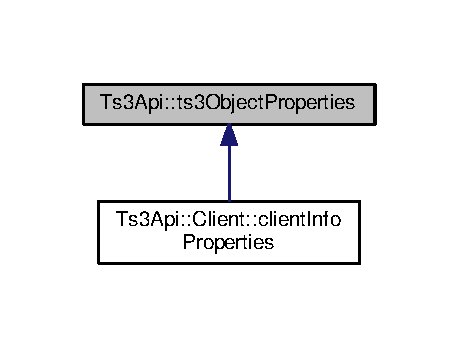
\includegraphics[width=220pt]{struct_ts3_api_1_1ts3_object_properties__inherit__graph}
\end{center}
\end{figure}


Collaboration diagram for Ts3\+Api\+:\+:ts3\+Object\+Properties\+:\nopagebreak
\begin{figure}[H]
\begin{center}
\leavevmode
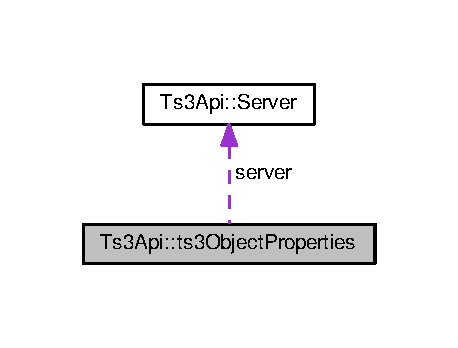
\includegraphics[width=220pt]{struct_ts3_api_1_1ts3_object_properties__coll__graph}
\end{center}
\end{figure}
\subsection*{Public Member Functions}
\begin{DoxyCompactItemize}
\item 
\hyperlink{struct_ts3_api_1_1property}{property} {\bfseries get\+Property} (string name)\hypertarget{struct_ts3_api_1_1ts3_object_properties_ae3cb0a412b4fa5ac6dc2b26e6431da2e}{}\label{struct_ts3_api_1_1ts3_object_properties_ae3cb0a412b4fa5ac6dc2b26e6431da2e}

\item 
{\bfseries ts3\+Object\+Properties} (\hyperlink{class_ts3_api_1_1_server}{Server} \&server, time\+\_\+t \&update\+Time, bool incomplete\+Init=false)\hypertarget{struct_ts3_api_1_1ts3_object_properties_afdb9693f8d6ebad8376edab2f355842f}{}\label{struct_ts3_api_1_1ts3_object_properties_afdb9693f8d6ebad8376edab2f355842f}

\end{DoxyCompactItemize}
\subsection*{Public Attributes}
\begin{DoxyCompactItemize}
\item 
map$<$ string, \hyperlink{struct_ts3_api_1_1property}{property} $>$ {\bfseries props\+Buff}\hypertarget{struct_ts3_api_1_1ts3_object_properties_af704b1184537ae8a377ca72cbb0450d7}{}\label{struct_ts3_api_1_1ts3_object_properties_af704b1184537ae8a377ca72cbb0450d7}

\item 
string {\bfseries data}\hypertarget{struct_ts3_api_1_1ts3_object_properties_aeb305dc4357f16608f5f9f248d52d0b5}{}\label{struct_ts3_api_1_1ts3_object_properties_aeb305dc4357f16608f5f9f248d52d0b5}

\item 
string {\bfseries command}\hypertarget{struct_ts3_api_1_1ts3_object_properties_a4446e3589a13aa75b0a5bad5e48cf879}{}\label{struct_ts3_api_1_1ts3_object_properties_a4446e3589a13aa75b0a5bad5e48cf879}

\item 
time\+\_\+t {\bfseries updated\+Time} = time(N\+U\+LL)\hypertarget{struct_ts3_api_1_1ts3_object_properties_a9ee07809dd901f74dfee84d4d09db7b6}{}\label{struct_ts3_api_1_1ts3_object_properties_a9ee07809dd901f74dfee84d4d09db7b6}

\item 
time\+\_\+t \& {\bfseries update\+Time}\hypertarget{struct_ts3_api_1_1ts3_object_properties_a65edbfaa26a0ca1de2ebdadfd354b3b4}{}\label{struct_ts3_api_1_1ts3_object_properties_a65edbfaa26a0ca1de2ebdadfd354b3b4}

\item 
\hyperlink{class_ts3_api_1_1_server}{Server} \& {\bfseries server}\hypertarget{struct_ts3_api_1_1ts3_object_properties_a564ab32932be4a0f35e25850fd3cf7a4}{}\label{struct_ts3_api_1_1ts3_object_properties_a564ab32932be4a0f35e25850fd3cf7a4}

\item 
bool {\bfseries incomplete\+Init} = false\hypertarget{struct_ts3_api_1_1ts3_object_properties_aa19c9df45dba9ab15832a33793414aec}{}\label{struct_ts3_api_1_1ts3_object_properties_aa19c9df45dba9ab15832a33793414aec}

\end{DoxyCompactItemize}
\subsection*{Protected Member Functions}
\begin{DoxyCompactItemize}
\item 
bool {\bfseries in\+Buff} (string name)\hypertarget{struct_ts3_api_1_1ts3_object_properties_a65236aa2fec0af870801637701718244}{}\label{struct_ts3_api_1_1ts3_object_properties_a65236aa2fec0af870801637701718244}

\item 
void {\bfseries clear\+Buff} ()\hypertarget{struct_ts3_api_1_1ts3_object_properties_ac9deae104a2f46f95a35482c90420dfb}{}\label{struct_ts3_api_1_1ts3_object_properties_ac9deae104a2f46f95a35482c90420dfb}

\item 
virtual void {\bfseries update} ()=0\hypertarget{struct_ts3_api_1_1ts3_object_properties_a83202a6c42ecdb30c89ce6240f25d69b}{}\label{struct_ts3_api_1_1ts3_object_properties_a83202a6c42ecdb30c89ce6240f25d69b}

\end{DoxyCompactItemize}


The documentation for this struct was generated from the following files\+:\begin{DoxyCompactItemize}
\item 
/home/karol/projects/\+Team\+Speak3-\/\+C-\/\+Query-\/\+A\+P\+I/src/includes/structs/ts3\+Object\+Properties.\+hpp\item 
/home/karol/projects/\+Team\+Speak3-\/\+C-\/\+Query-\/\+A\+P\+I/src/ts3\+Object\+Properties.\+cpp\end{DoxyCompactItemize}

\hypertarget{struct_ts3_api_1_1ts3_response}{}\section{Ts3\+Api\+:\+:ts3\+Response Struct Reference}
\label{struct_ts3_api_1_1ts3_response}\index{Ts3\+Api\+::ts3\+Response@{Ts3\+Api\+::ts3\+Response}}
\subsection*{Public Member Functions}
\begin{DoxyCompactItemize}
\item 
{\bfseries ts3\+Response} (string data=\char`\"{}\char`\"{}, string error\+Id=\char`\"{}0\char`\"{}, string error\+Msg=\char`\"{}\char`\"{})\hypertarget{struct_ts3_api_1_1ts3_response_a042b64ba362ee4c20abeb5b1019a4f2e}{}\label{struct_ts3_api_1_1ts3_response_a042b64ba362ee4c20abeb5b1019a4f2e}

\item 
string {\bfseries message\+Decode} (string message)\hypertarget{struct_ts3_api_1_1ts3_response_ab86f3de75a74609f5d193593bc5dcd75}{}\label{struct_ts3_api_1_1ts3_response_ab86f3de75a74609f5d193593bc5dcd75}

\item 
string {\bfseries message\+Encode} (string message)\hypertarget{struct_ts3_api_1_1ts3_response_a389f5213e2e3c28e6dd23cd035b954ce}{}\label{struct_ts3_api_1_1ts3_response_a389f5213e2e3c28e6dd23cd035b954ce}

\end{DoxyCompactItemize}
\subsection*{Public Attributes}
\begin{DoxyCompactItemize}
\item 
string {\bfseries data} = \char`\"{}\char`\"{}\hypertarget{struct_ts3_api_1_1ts3_response_aa3ed5cc6cc00af0631109af4cc1537b9}{}\label{struct_ts3_api_1_1ts3_response_aa3ed5cc6cc00af0631109af4cc1537b9}

\item 
string {\bfseries error\+Id} = \char`\"{}0\char`\"{}\hypertarget{struct_ts3_api_1_1ts3_response_a5d1bfb46754667196c77d5b8cb0fc00f}{}\label{struct_ts3_api_1_1ts3_response_a5d1bfb46754667196c77d5b8cb0fc00f}

\item 
string {\bfseries error\+Msg} = \char`\"{}\char`\"{}\hypertarget{struct_ts3_api_1_1ts3_response_a49ce712e761bd347b69c2a3bdf827e57}{}\label{struct_ts3_api_1_1ts3_response_a49ce712e761bd347b69c2a3bdf827e57}

\item 
bool {\bfseries error} = true\hypertarget{struct_ts3_api_1_1ts3_response_a07b75d89c300e345763933e062c5777f}{}\label{struct_ts3_api_1_1ts3_response_a07b75d89c300e345763933e062c5777f}

\end{DoxyCompactItemize}


The documentation for this struct was generated from the following files\+:\begin{DoxyCompactItemize}
\item 
/home/karol/projects/\+Team\+Speak3-\/\+C-\/\+Query-\/\+A\+P\+I/src/includes/structs/server\+Structs.\+hpp\item 
/home/karol/projects/\+Team\+Speak3-\/\+C-\/\+Query-\/\+A\+P\+I/src/server\+Structs.\+cpp\end{DoxyCompactItemize}

%--- End generated contents ---

% Index
\backmatter
\newpage
\phantomsection
\clearemptydoublepage
\addcontentsline{toc}{chapter}{Index}
\printindex

\end{document}
